\documentclass[oneside, aspectratio=169]{beamer}

%\usepackage{scrextend}
%\changefontsizes{13pt}
\linespread{1.2} % Giãn dòng
\setlength{\parskip}{\baselineskip} % Khoảng cách giữa các đoạn
\usepackage[skip=6pt, indent=1cm]{parskip} % Tùy chỉnh cách đoạn và thụt đầu dòng
\usepackage{setspace}
\usepackage[utf8]{vietnam}
%\usepackage[linesnumbered, commentsnumbered]{algorithm2e}
\usepackage{appendixnumberbeamer}
\usepackage{mathptmx}

\usepackage{multirow}
\usepackage{makecell}
\usepackage{verbatim}


\usepackage[sorting=none,style=numeric,backend=bibtex]{biblatex}
\bibliography{reflib.bib}
%\usepackage{beamerthemesplit} 
\setbeamertemplate{footline}[frame number]
\setbeamertemplate{headline}{}
\usepackage{pgfplots}
\pgfplotsset{compat=newest}
\usepackage{booktabs}
%%%%%%%%%%%%%%%%%%
\definecolor{CTUcyan}{rgb}{0, 0.6862745098039216, 0.9372549019607843}
\definecolor{CTUblue}{rgb}{0.121568627450, 0.3607843137254902, 0.6627450980392157}

\usepackage{amsfonts,amsmath,amssymb,bm}
\usepackage{algorithm}
\usepackage{algorithmicx}
\usepackage{verbatim}
\usepackage{graphicx}
\usepackage{subcaption}
\usepackage{booktabs,multicol,calligra}  %Allows the use of \toprule, \midrule and \bottomrule in tables
\usepackage{hyperref}
\usepackage{tcolorbox}
\usetikzlibrary{arrows,shapes}
\usepackage{multicol}
\usepackage{animate}

\newcommand{\bluenum}[1]{%
	\tikz[baseline=(char.base)]{
		\node[shape=circle, draw=none, fill=CTUblue, text=white,
		inner sep=0.1pt, minimum size=12pt,
		font=\bfseries\scriptsize] (char) {#1};
	}%
}





\mode<presentation>
{
	
	\setbeamertemplate{background canvas}{
		\begin{tikzpicture}
			\path (0,0) -- (\paperwidth,\paperheight);
			\node[opacity=.05] at (0.5\paperwidth,0.45\paperheight)
			{
\includegraphics[width=6cm]{BG/CTU_logo_singlecolor}};
		\end{tikzpicture}
	}
	
	\useinnertheme[shadow]{rounded}
	\usefonttheme{serif}
	\setbeamerfont{footnote}{size=\tiny} % hoặc \tiny, \footnotesize, \small, \normalsize
	
	\useinnertheme{circles}
	\setbeamertemplate{navigation symbols}{}
	\setbeamertemplate{caption}[numbered]
	\setbeamercolor*{palette tertiary}{use=structure,bg=CTUblue}
	\setbeamercolor*{palette quaternary}{fg=white,bg=CTUblue}
	\setbeamercolor{frametitle}{fg=CTUblue}
	\setbeamercolor{title}{fg=CTUblue}
	
	\setbeamercolor{block title}{bg=CTUblue, fg=white}
	\setbeamerfont{block title}{size=\small,series=\bfseries}
	
	\setbeamerfont*{frametitle}{size=\large,
		series=\bfseries,
		parent=structure}
	\setbeamercolor{block body}{bg=CTUblue!10}
	\setbeamercolor{section in toc}{fg=white}
	\setbeamercolor{subsection in toc}{fg=white}
	
	\setbeamertemplate{headline}{
		\begin{tikzpicture}[remember picture, overlay]
			% Thanh màu
			\fill[CTUcyan] (current page.north west) rectangle ([xshift=.7\paperwidth,yshift=-0.1cm]current page.north west);
			\fill[CTUblue] ([xshift=.7\paperwidth]current page.north west) rectangle ([xshift=\paperwidth,yshift=-0.1cm]current page.north west);
		\end{tikzpicture}
	}
	%	
}



\beamertemplatenavigationsymbolsempty


\title[]{\textbf{\color{white} Báo cáo luận văn tốt nghiệp thạc sĩ}}
\subtitle{\normalsize\color{white}Nhận dạng thống kê cho hàm mật độ xác suất mất~cân~bằng và ứng dụng cho ảnh \\\rule{3cm}{2pt}}
\author[HUNG Tran-Nam]{\color{white}\normalsize Trần Nam Hưng\inst{1}}
\institute[CTU]{\color{white}\footnotesize
	\inst{1} Khoa Khoa học Tự nhiên, Trường Đại học Cần Thơ
}
\date[Oct 26, 2025]{\color{white}\footnotesize Ngày 26 tháng 10 năm 2025}

%\AtBeginSection[ ]
%{	
%	\usebackgroundtemplate{
\includegraphics[width=\paperwidth]{BG/thank2.pdf}}%
%			\begin{frame}
%						{\Large\bf\color{white} Mục lục}}
%						\tableofcontents[currentsection]
%					\end{frame}
%		}


\begin{document}
	
{
	\usebackgroundtemplate{
		
\includegraphics[width=\paperwidth,height=\paperheight]{BG/thank2.pdf}
	}
	\begin{frame}[plain]
		\vspace{1.8cm}
		{\color{white}
		\titlepage
		}
	\end{frame}
}
	
	{
		\usebackgroundtemplate{
\includegraphics[width=\paperwidth]{BG/thank2.pdf}}%
		\begin{frame}[plain]{}
			\vspace{3em}
\begin{center}
	\large\bf\color{white} NỘI DUNG CHÍNH
\end{center}
\centering
\begin{minipage}{.9\textwidth}
	\begin{enumerate}
		\item {\color{white} PHẦN MỞ ĐẦU}
		\item {\color{white} PHẦN NỘI DUNG}
			\begin{enumerate}
			\item {\color{white} Chương 1. Một số vấn đề liên quan đến hàm mật độ xác suất}
			\item {\color{white} Chương 2. Nhận dạng thống kê cho dữ liệu mất cân bằng}
			\item {\color{white} Chương 3. Ứng dụng cho dữ liệu hình ảnh}
		\end{enumerate}
		\item {\color{white} PHẦN KẾT LUẬN}
		\item {\color{white} TÀI LIỆU THAM KHẢO}
	\end{enumerate}
\end{minipage}
		\end{frame}
	}


	{
	\usebackgroundtemplate{
\includegraphics[width=\paperwidth]{BG/thank2.pdf}}%
	\begin{frame}[plain]{}
		\vspace{1em}
		\begin{center}
			\large\bf\color{white} PHẦN MỞ ĐẦU
		\end{center}
		\centering
		\begin{minipage}{.7\textwidth}
			\color{white}
			\begin{enumerate}
				\item {\color{white} Lý do chọn đề tài}
				\item {\color{white} Mục đích nghiên cứu}
				\item {\color{white} Đối tượng nghiên cứu}
				\item {\color{white} Phương pháp nghiên cứu và cấu trúc luận văn}
			\end{enumerate}
		\end{minipage}
	\end{frame}
}


%
\begin{frame}{1. Lý do chọn đề tài}{\textbf{\bluenum{1} SR là kiến thức nền tảng của AI dự đoán}}
	
	\begin{figure}
		\centering
		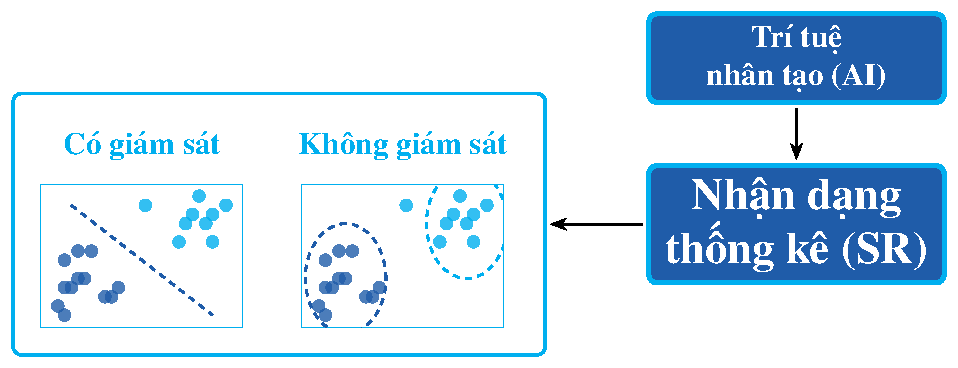
\includegraphics[width=.8\textwidth]{Figs/lydochondetai1}
	\end{figure}
	
\end{frame}
%
\begin{frame}{1. Lý do chọn đề tài}{\textbf{\bluenum{2} SR cho các PDF là khách thể mới cần giải quyết}}
	
	\begin{figure}
		\centering
		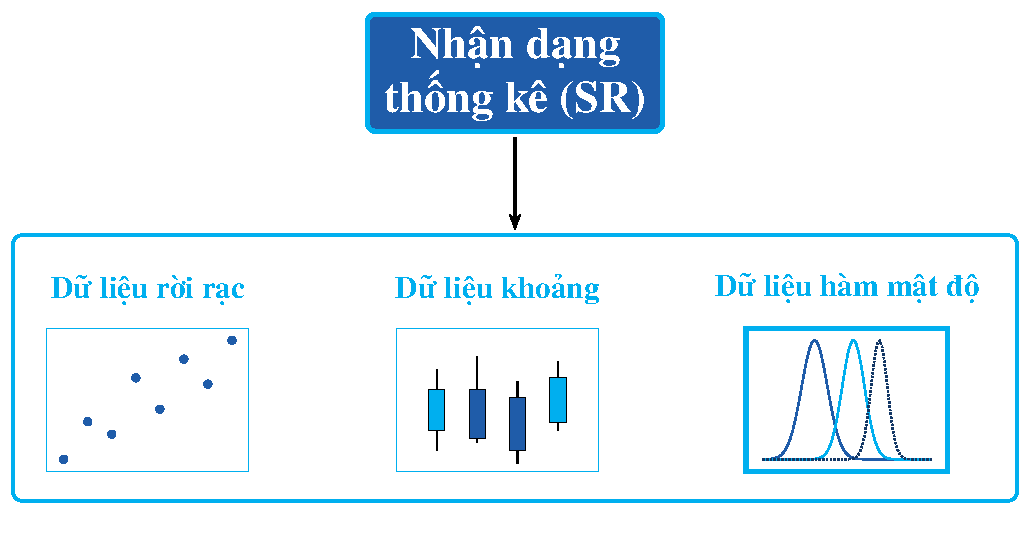
\includegraphics[width=.8\linewidth]{Figs/lydochondetai2}
	\end{figure}
	{\color{CTUblue}
		$\Rightarrow$ Dữ liệu PDF cho ta thông tin mật độ, độ lệch, phân tán. Nó là một khách thể nghiên cứu.}
	
\end{frame}

\begin{frame}{1. Lý do chọn đề tài}{\textbf{\bluenum{3} SR truyền thống cho PDF bị thiên lệch với mất cân bằng}}
	
	\begin{figure}
		\centering
		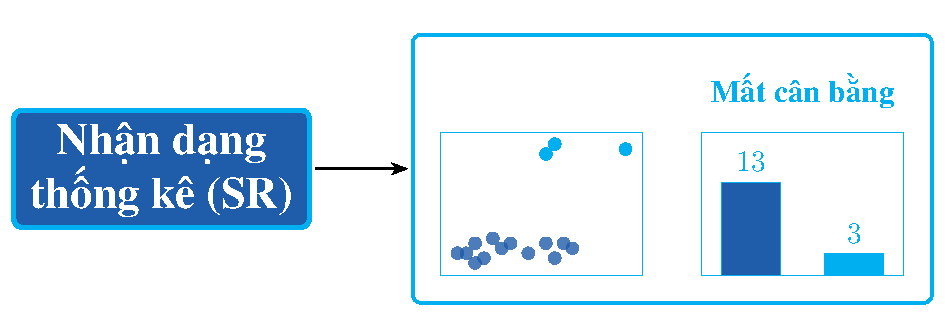
\includegraphics[width=.8\textwidth]{Figs/lydochondetai3}
	\end{figure}
	
\end{frame}




\begin{frame}{1. Lý do chọn đề tài}{	``Nhận dạng thống kê cho~hàm~mật~độ~xác~suất mất~cân~bằng và~ứng dụng cho dữ liệu ảnh''}
	
	\begin{figure}
		\centering
		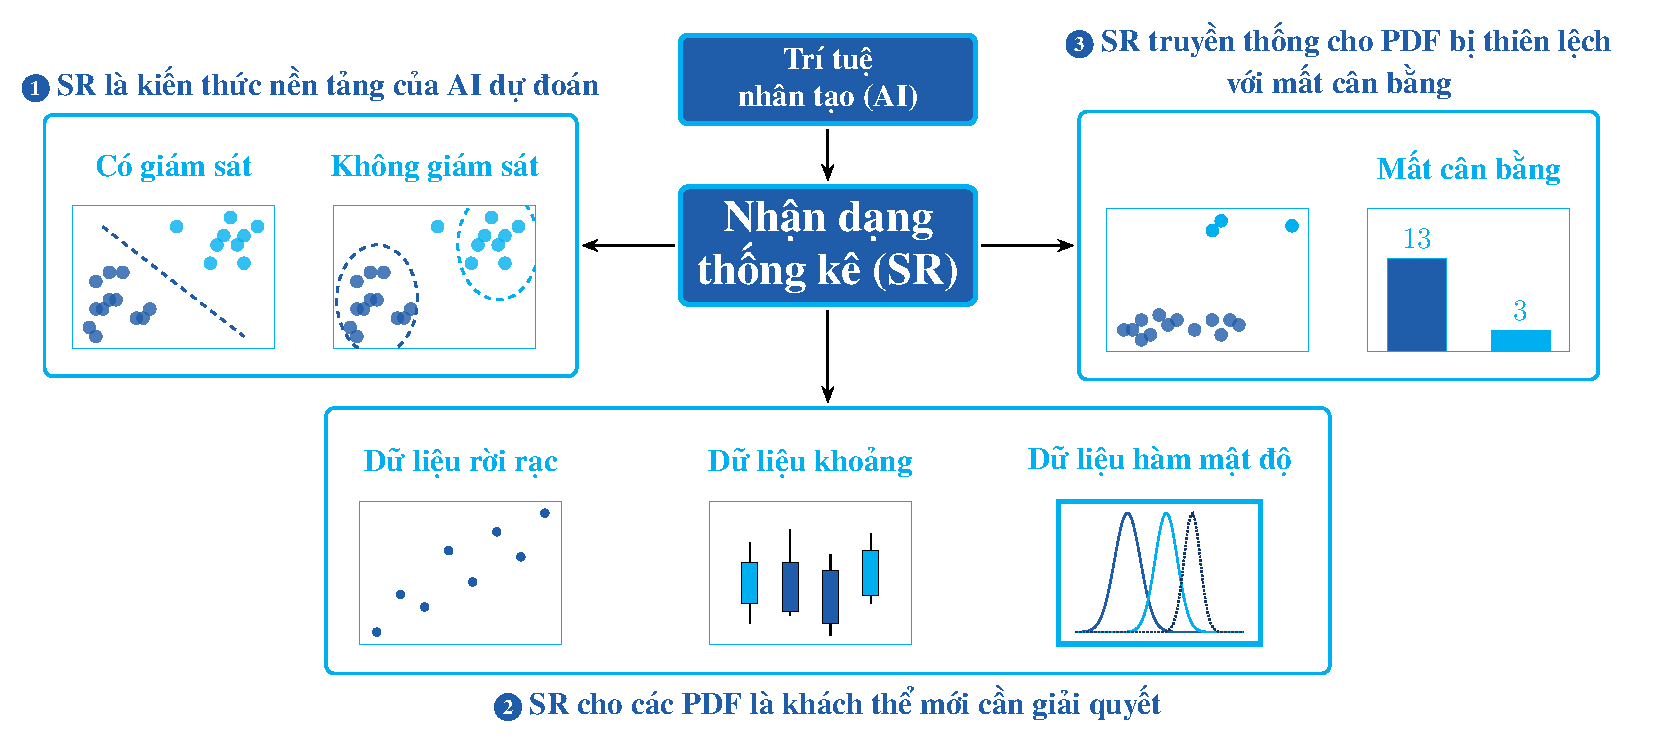
\includegraphics[width =\linewidth]{Figs/lydochondetai}
	\end{figure}

\end{frame}

\begin{frame}{2. Mục đích và phạm vi nghiên cứu}\footnotesize
	
	\begin{columns}[t,onlytextwidth]
		
		% ===== CỘT TRÁI =====
		\begin{column}{0.48\textwidth}
			
			\begin{block}{Khoảng trống nghiên cứu}
				\begin{enumerate}
					\item \textit{Khoảng trống lý thuyết:} Chưa xây dựng khung lý thuyết đầy đủ cho bài toán SR trên PDF mất cân bằng dữ liệu;
					\item \textit{Khoảng trống thực nghiệm:} Chưa có nhiều thử nghiệm ứng dụng phân tích hình ảnh thông qua đại diện PDF cho bài toán SR mất cân bằng.
				\end{enumerate}
			\end{block}
			
						\begin{block}{Đối tượng nghiên cứu}
				\begin{enumerate}
					\item Thuật toán phân loại và phân tích chùm trong điều kiện dữ liệu mất cân bằng;
					\item Dữ liệu hình ảnh được trích xuất và biểu diễn dưới dạng PDF đại diện.
				\end{enumerate}
			\end{block}
			
		\end{column}
		
		% ===== CỘT PHẢI =====
		\begin{column}{0.48\textwidth}
			
	\begin{block}{Mục đích nghiên cứu}
	\begin{enumerate}
		\item \textcolor{CTUblue}{\textit{Xây dựng thuật toán}} phân loại và phân tích chùm PDF có mất cân bằng;
		\item \textcolor{CTUblue}{\textit{Áp dụng phân tích hình ảnh}} với các đặc trưng được trích xuất và đại diện bởi PDF để nhận dạng.
	\end{enumerate}
\end{block}
			
			\begin{block}{Phạm vi nghiên cứu}
				\begin{enumerate}
					\item Các thuật toán phân tích chùm và phân loại cho PDF;
					\item Dữ liệu hình ảnh được trích xuất thành PDF đại diện;
					\item Các vấn đề tính toán liên quan đến các phương pháp SR.
				\end{enumerate}
			\end{block}
			
		\end{column}
		
	\end{columns}
	
\end{frame}




\begin{frame}{3. Phương pháp và cấu trúc}
	
	\begin{columns}   
		\begin{column}{.6\textwidth}
				\begin{block}{Phương pháp nghiên cứu}
						\begin{enumerate}
						\item {\it\color{CTUblue} Nghiên cứu lý thuyết:} Phân tích -- tổng~kết, phân loại  -- hệ thống hóa kiến thức về lĩnh vực SR; So sánh đánh giá ưu điểm và nhược điểm của các thuật toán.
						\item {\it\color{CTUblue} Thực nghiệm khoa học:} Thực hiện các ví~dụ~số minh họa lý thuyết trong môi trường mô phỏng; xử lý so sánh kết quả bằng các phân tích thống kê.
					\end{enumerate}
				\end{block}
		\end{column}
		\begin{column}{.4\textwidth}
					\begin{figure}
				\centering
				
\includegraphics[width=\textwidth]{Figs/mindchart}
			\end{figure}
		\end{column}
	\end{columns}
	

\end{frame}







{
	\usebackgroundtemplate{
\includegraphics[width=\paperwidth]{BG/thank2.pdf}}%
	\begin{frame}[plain]{}
		\vspace{1em}
		\begin{center}
			\large\bf\color{white} PHẦN NỘI DUNG
		\end{center}
		\centering
		\begin{minipage}{.7\textwidth}
			\color{white}
			\begin{enumerate}
				\item {\color{white} Một số vấn đề liên quan đến hàm mật độ xác suất}
				\item {\color{white} Nhận dạng thống kê cho hàm mật độ xác suất với dữ liệu mất cân bằng}
				\item {\color{white} Ứng dụng cho dữ liệu hình ảnh}
			\end{enumerate}
		\end{minipage}
	\end{frame}
}

\begin{frame}{1.1. Hàm mật độ xác suất (PDF)}\small
\begin{columns}
	\begin{column}{.5\textwidth}
			\begin{figure}
			\centering
			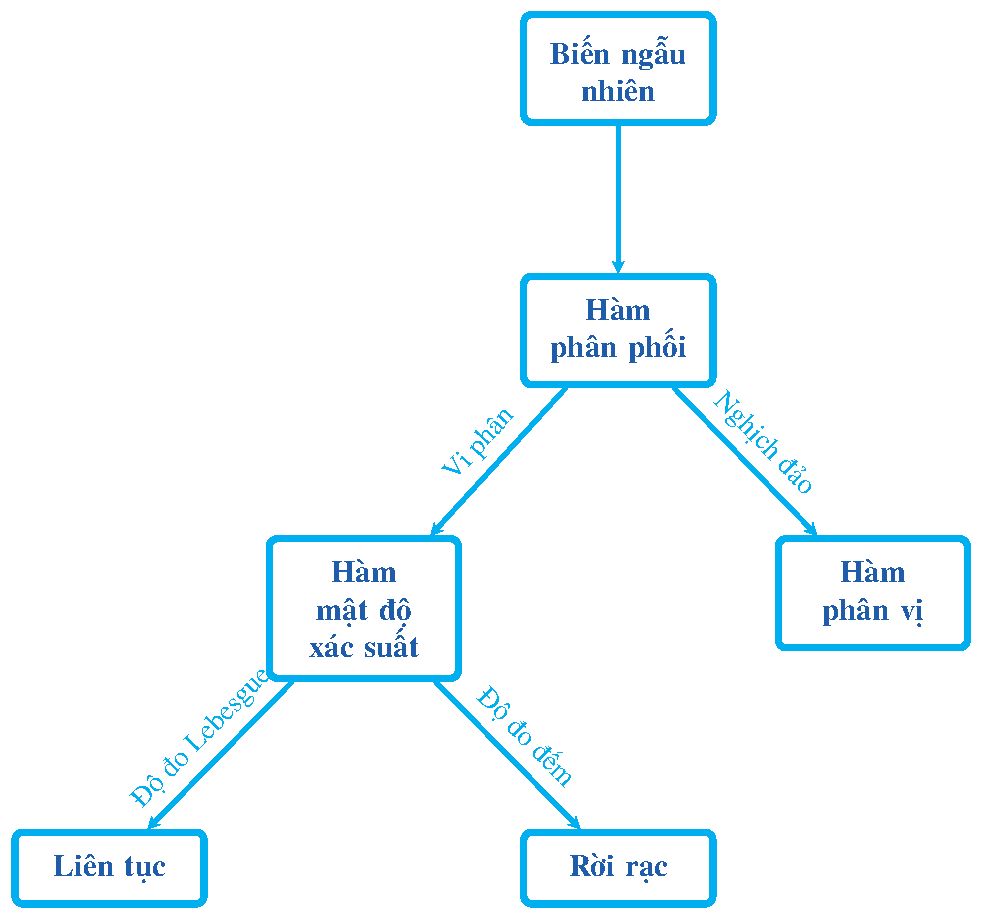
\includegraphics[width=.85\textheight]{Figs/hammatdoxacsuat}
		\end{figure}

	\end{column}
	\begin{column}{.5\textwidth}
			\begin{definition}[Dữ liệu PDF $1$-chiều]\label{dng:data1}
			Dữ liệu PDF một bộ đối tượng không chắc chắn $o$ có dạng $(o_1\,;o_2\,;\ldots\,;o_n)$ \cite{gullo2008hierarchical}. Mỗi đối tượng $o_j$ chứa một cặp $(I_j\,;f_j)$ với mỗi $1\le j\le n$, trong đó $I_j=[l_j\,;u_j]$ là khoảng xác định của $o_j$ và $f\,:\,\mathbb{R}\to\mathbb{R}^+$ là PDF xếp các giá trị xác suất vào mỗi $x\in I_j$ sao cho 
			$$\int_{x\in I_j}f_j(x)\mathrm{\,d}x=1 \text{ và } \int_{x \in\mathbb{R}\setminus I_j}f_j(x)\mathrm{\,d}x=0. $$
		\end{definition}
	\end{column}
\end{columns}
\end{frame}

\begin{frame}{1.2. Hàm mật độ xác suất bổ sung}
	
	\begin{columns}
		\begin{column}{.6\textwidth}
			
			\begin{definition}[PDF đại diện chùm]\footnotesize
				Cho tập $\mathcal{F}$ gồm $n$-PDF với $n\ge 2$. Ta phân bổ $\mathcal{F}$ vào $c$-chùm, với $1<c\le n$. Khi đó, PDF đại diện của các chùm $c_i$ là 
				\begin{align}\label{daidien}
					\theta_i(x) = \frac{\sum_{j=1}^n\mu_{ij}\times f_j(x)}{\sum_{j=1}^n\mu_{ij}},
				\end{align}
				trong đó $\mu_{ij}$ là trọng số phân bổ một PDF $f_j(x)$ bất kỳ vào tập hợp hàm \footnote[frame]{\fullcite{nguyentrang2017fuzzy}}.
			\end{definition}
		\end{column}
		\begin{column}{.4\textwidth}
			\begin{figure}
				\centering
				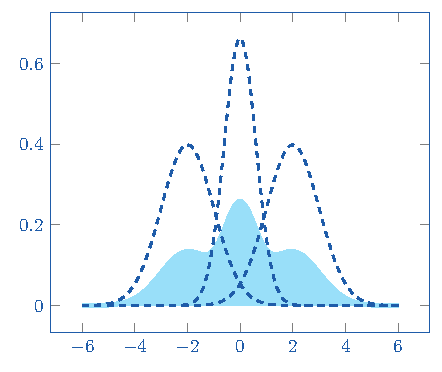
\includegraphics[width=\textwidth]{Figs/daidienchum1}
			\end{figure}
		\end{column}
	\end{columns}
	
\end{frame}


\begin{frame}{1.2. Hàm mật độ xác suất bổ sung (t.t.)}
	
	\begin{columns}
		\begin{column}{.6\textwidth}
			
			\begin{definition}[PDF đại diện Gauss]\footnotesize
		Một PDF đại diện Gauss có dạng phân phối chuẩn sao cho tổng khoảng cách giữa chúng đến các PDF khác là nhỏ nhất \cite{frechet1948elements,nguyen2023balance,nguyen2023globally}, tức là
				$$\theta_i(x) = \arg\min_{\mathcal{N}(\mu\,;\sigma)}\sum_{j=1}^n\mu_{ij}D(\mathcal{N}(\mu\,;\sigma)\,;f_j(x)),$$
				trong đó $D(\mathcal{N}(\mu\,;\sigma)\,;f_j(x))$ là khoảng cách giữa một PDF Gauss đến tất cả các PDF $f_j(x)$ khác trong tập hợp hàm\footnote[frame]{\fullcite{nguyen2023globally};\\\fullcite{nguyen2023balance}}.
			\end{definition}
		\end{column}
		\begin{column}{.4\textwidth}
			\begin{figure}
				\centering
				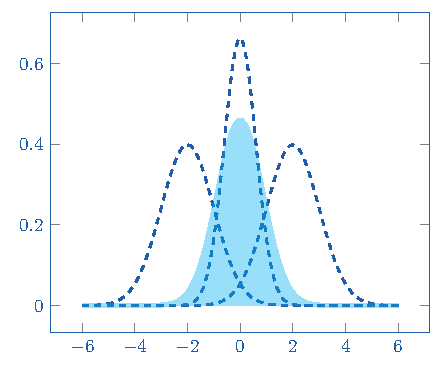
\includegraphics[width=\textwidth]{Figs/daidienchum2}
			\end{figure}
		\end{column}
	\end{columns}
	
	
\end{frame}


\begin{frame}{1.3. Độ đo khoảng cách hai PDF}{Ví dụ 1.1}
			\begin{columns}
				
				\begin{column}{.5\textwidth}
					
					\begin{figure}
						\centering
						
\includegraphics[width=.9\textwidth]{Figs/C1_Uniform.pdf}
					\end{figure}
					
				\end{column}
				
				\begin{column}{.5\textwidth}
					
					\begin{table}
						\centering\scriptsize
						\begin{tabular}{llcccc}
							\toprule
							&                                 &    (a)     &    (b)    &    (c)     &    (d)     \\ \midrule
							\multirow{3}{*}{Họ $\mathcal{L}_p$} & $\mathcal{L}_1$                 &   2{,}0   &  2{,}0   &   2{,}0   &   1{,}0   \\
							& $\mathcal{L}_2$                 &   1{,}4   &  1{,}2   &   1{,}4   &   0{,}7   \\
							& $D_O$             &   1{,}0   &  1{,}0   &   1{,}0   &   0{,}5   \\
							& $CWD$                           &   1{,}0   &  1{,}0   &   1{,}0   &   0{,}5   \\ \midrule
							\multirow{6}{*}{Họ  $f$}    & $D_{BC}$      &  $\infty$  & $\infty$  &  $\infty$  &   0{,}7   \\
							& $D^2_H$         &   1{,}0   &  1{,}0   &   1{,}0   &   0{,}7   \\
							& $D_M$                &   1{,}4   &  1{,}4   &   1{,}4   &   1{,}0   \\
							& $D_{KL}$  &  27{,}6   &  27{,}3  &  27{,}6   &  13{,}5   \\
							& $D_{JS}$   &  27{,}6   &  26{,}9  &  27{,}6   &  13{,}5   \\ \midrule
							Họ Optimal                          & $W_2^2$      & \bf 3{,}0 & \bf 3{,}5 & \bf 6{,}0 & \bf 1{,}0 \\ \bottomrule
						\end{tabular}
					\end{table}
					
				\end{column}
			\end{columns}
			
\end{frame}


\begin{frame}{1.4. Độ đo khoảng cách chùm PDF}
	
	
	\begin{figure}
		\centering
		
\includegraphics[width=\linewidth]{Figs/C1_Linkage.pdf}
	\end{figure}
	
	
	\begin{table}[H]
		\centering\footnotesize
		\begin{tabular*}{\columnwidth}{@{\extracolsep\fill}lll@{\extracolsep\fill}} 
			\toprule
			\bf Liên kết &\bf Ký hiệu & \bf                             $\Delta$                             \\ \midrule
		(a)	Liên kết đơn\footnotemark[1] (SLINK)\cite{florek1951liaison}&$\Delta_{\min}$&$\min_{f\in\mathcal{F}, g\in\mathcal{G}}D(f\,;g)$\\
		(b)	Liên kết đủ\footnotemark[2] (CLINK)\cite{sorensen1948method} &$\Delta_{\max}$& $\max_{f\in\mathcal{F}, g\in\mathcal{G}}D(f\,;g)$\\
		(c)	Liên kết tâm (UPGMC)&$\Delta_{centroid}$&$D(\theta_{\mathcal{F}}\,;\theta_{\mathcal{G}})$\\
		(d)	Liên kết trung bình (UPGMA)&$\Delta_{avg}$ & $\frac{1}{\#\mathcal{F}\#\mathcal{G}}\sum_{f\in\mathcal{F}, g\in\mathcal{G}}D(\mathcal{F}\,;\mathcal{G})$\\
		(e)	Liên kết Ward \cite{ward1963hierarchical}&$\Delta_{Ward}$ &$\frac{\#\mathcal{F} \cdot \#\mathcal{G}}{\#\mathcal{F} + \#\mathcal{G}} D^2\big(\theta_{\mathcal{F}}\,;\theta_{\mathcal{G}}\big)
			$\\ \bottomrule
		\end{tabular*}
	\end{table}
	
\end{frame}



\begin{frame}{1.5. Phân tích chùm hàm mật độ xác suất} {Phân tích chùm không mờ (KCF \& HCF)}
	
Bài toán phân tích chùm phân bổ PDF thứ $j$ vào chùm thứ $i$ trong $c$-chùm cho trước với $i=1\,,2\,,\ldots\,,c$ và $c\in\mathbb{N}$, thỏa mãn ba ràng buộc
	\begin{enumerate}\footnotesize
		\item Hợp tất cả các chùm $\bigcup_i c_i$ bằng $\mathcal{F}$;
		\item Giao của mỗi chùm là rỗng, tức là $c_i\cap c_j =\emptyset$, với mỗi $i\ne j$;
		\item Lực lượng của mỗi chùm là khác rỗng, tức là $|c_i|\ne \emptyset$.
	\end{enumerate}
	
	
	Phân tích chùm KCF là bài toán tối tiểu đơn mục tiêu cho tổng các bình phương khoảng cách trong chùm các PDF. \cite{macqueen1967some,Tai2010,nguyen2024new}, tức là
	\begin{align}\tag{KCF}\label{Jk}
		\text{Minimise}\,&:\, J(\bm U\,; \Theta\,|\, \mathcal{F}\,;c) = \sum_{i=1}^{c}\sum_{f_j(x)\in c_i}\mu_{ij}{D}^2(\theta_i\,;{f}_j),
	\end{align}
{\footnotesize	trong đó hàm $\theta_i(x)$ là PDF trọng tâm của chùm thứ $c_i$ và $\mu_{ij} =1$ nếu PDF $f_j$ thuộc chùm $c_i$ và $\mu_{ij}=0$ nếu ngược lại. }
	
	
\end{frame}

\begin{frame}{1.6. Phân tích chùm hàm mật độ xác suất} {Phân tích chùm không mờ (KCF \& HCF)}
		Cho bảy PDF Gauss $1$-chiều $\mathcal{F}$ cho bởi Tai Vo-Van \& Pham-Gia, T., (2010) \cite{Tai2010} có phương sai đồng nhất $\sigma_i^2 = 1$, với $i = 1\,;2\,;\ldots\,;7$ và các trung bình lần lượt là $\mu_i = \{0{,}3\,;4{,}0\,;9{,}1\,;1{,}0\,;5{,}5\,;8{,}0\,;4{,}8\}.$ Phân tích chùm KCF với $c=3$ và khoảng cách xét là $\mathcal{L}_2$.
	
	\begin{figure}
		\centering
		\begin{subfigure}[b]{.45\textwidth}
			\centering
			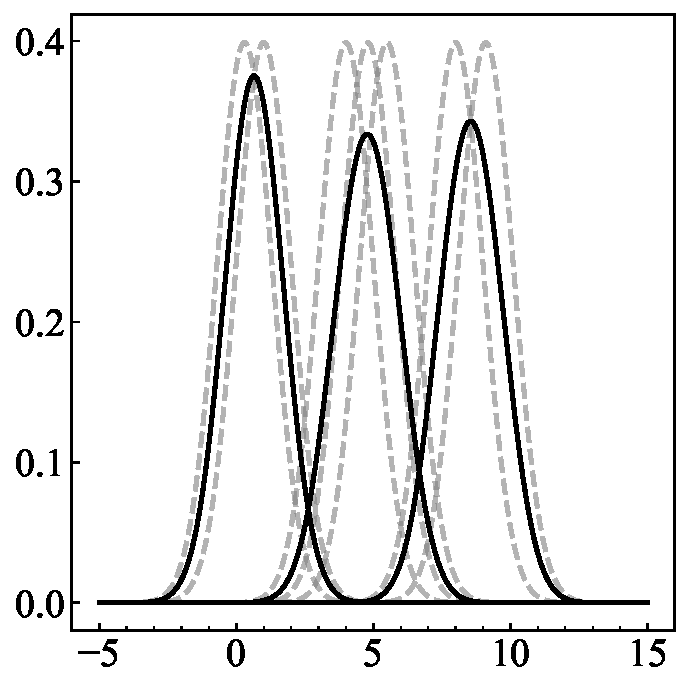
\includegraphics[width=.6\linewidth]{Figs/KCF_L2}
			\caption{Trọng tâm chùm}
		\end{subfigure}
		\begin{subfigure}[b]{.45\textwidth}
			\centering
			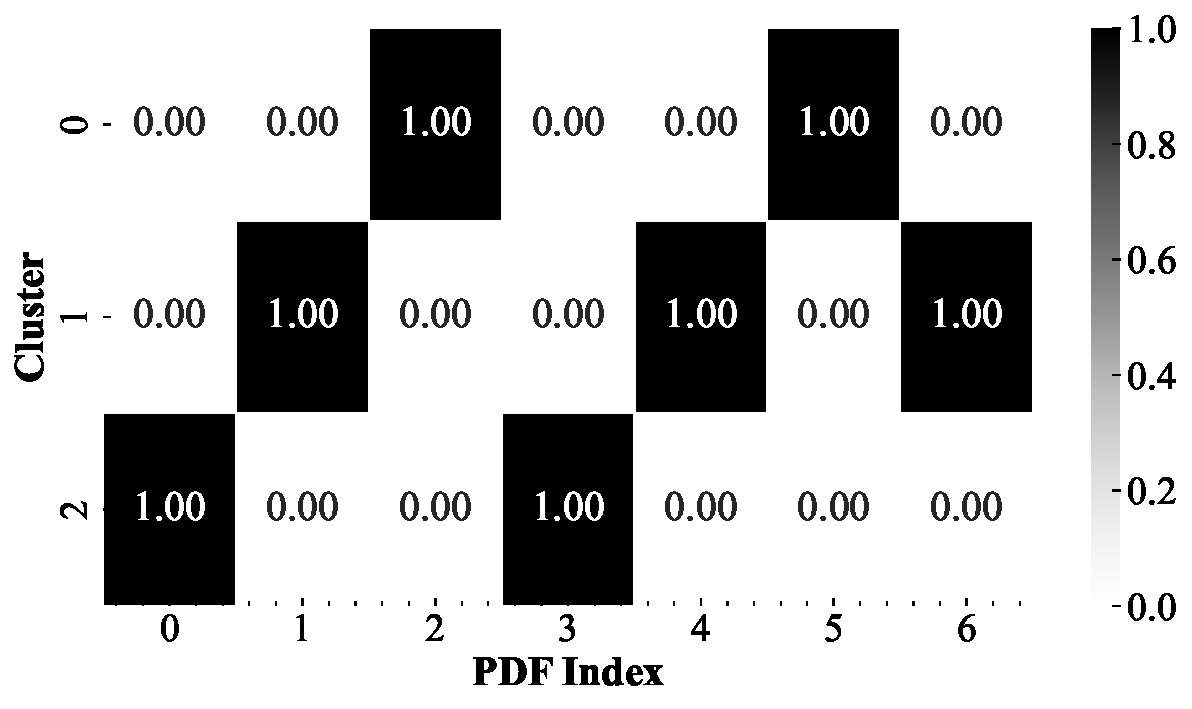
\includegraphics[width=\linewidth]{Figs/KCF_U}
			\caption{Ma trận phân vùng}
		\end{subfigure}
	\end{figure}
	
\end{frame}


\begin{frame}{1.6. Phân tích chùm hàm mật độ xác suất} {Phân tích chùm không mờ (KCF \& HCF)}
	
	\begin{figure}[H]
		\centering
		\begin{subfigure}[b]{.45\textwidth}
			\centering
			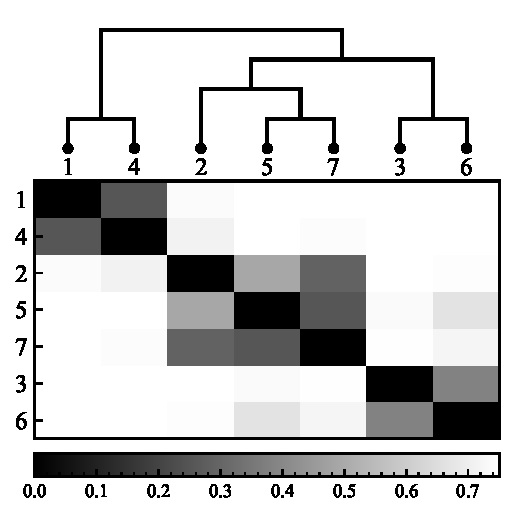
\includegraphics[width=.8\linewidth]{Figs/tree_L2_complete.pdf}
			\caption{Liên kết đủ}
		\end{subfigure}
		\begin{subfigure}[b]{.45\textwidth}
			\centering
			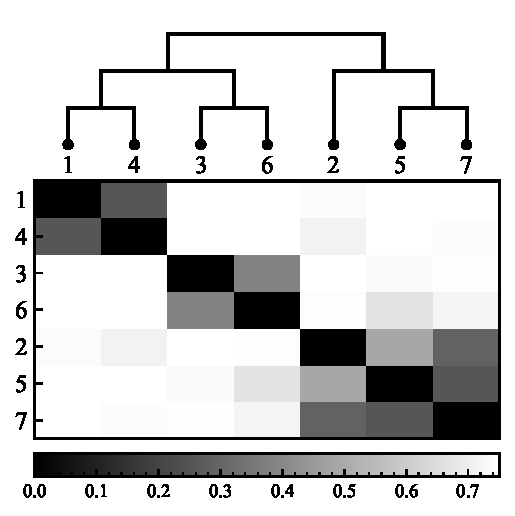
\includegraphics[width=.8\linewidth]{Figs/tree_L2_ward.pdf}
			\caption{Liên kết Ward}
		\end{subfigure}
		
	\end{figure}
{\color{CTUblue}\small Phương pháp liên kết đủ có xu hướng tạo ra các chùm nhỏ, có thứ tự. Ngược lại, liên kết Ward cho kết quả các chùm có tính đồng nhất cao hơn về phân bố, làm cây phân cấp cân đối.}

\end{frame}



\begin{frame}{1.6. Phân tích chùm hàm mật độ xác suất} {Phân tích chùm mờ (FCF)}
\begin{columns}
	\begin{column}{.5\textwidth}\footnotesize
			Giả sử $\mathcal{F}$-PDF chưa được gán nhãn, mục tiêu của bài toán là tối tiểu hóa tổng trọng số các giá trị hàm thành viên $\bm\mu$ có trọng số và bình phương khoảng cách $D(\theta_i\,;f_j)$.
		\begin{align}\tag{FCF}\label{Jf}
			\text{Minimise}\,&:\, J(\bm U\,;\Theta\,|\, \mathcal{F}\,;c\,;m) = \sum_{i=1}^{c}\sum_{j=1}^{n}\mu_{ij}^m{D}^2(\theta_i\,;{f}_j),\\\nonumber
			\text{s.t}\,&:\,\sum_{i=1}^{c} \mu_{ij} = 1,\quad \forall j \in \{1\,,2\,, \ldots\,, n\}, \tag{C1}\label{c1} \\
			\,&\mu_{ij} \in [0\,;1],\quad \forall i \in \{1\,,2\,,\ldots\,,c\}, \forall j \in \{1\,,2\,,\ldots\,,n\}, \tag{C2}\label{c2} \\
			\,&\sum_{j=1}^{n} \mu_{ij} > 0,\quad \forall i \in {1\,,2\,,\ldots\,,c}. \tag{C3}\label{c3}
		\end{align}	
	\end{column}
	\begin{column}{.5\textwidth}
		\begin{figure}[H]
	\centering
	
\includegraphics[width=\linewidth]{Figs/C1_phanvung.pdf}
\end{figure}
		\begin{figure}[H]
	\centering
	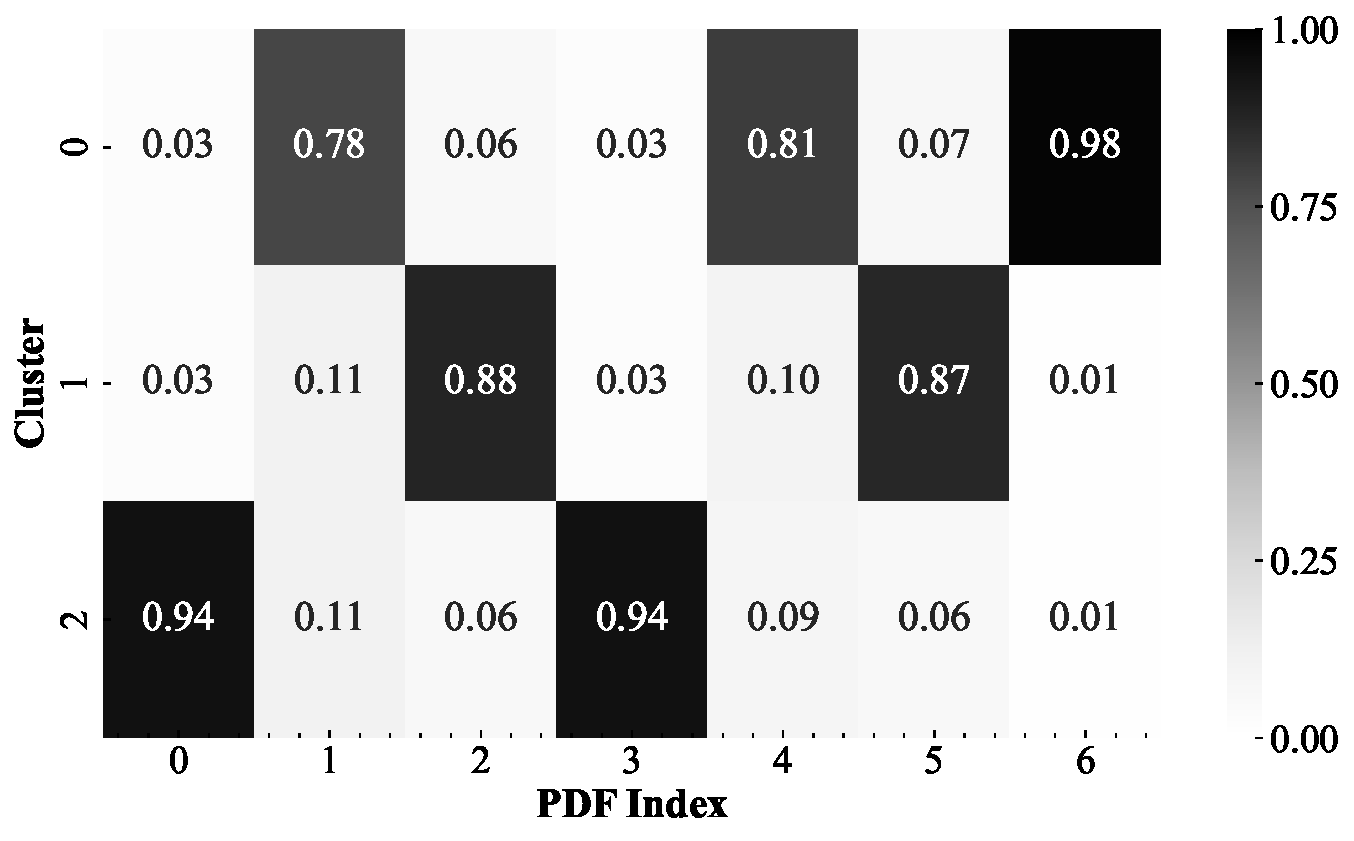
\includegraphics[width=\linewidth]{Figs/FCF_U9.pdf}
\end{figure}
	\end{column}
\end{columns}
	
\end{frame}


\begin{frame}{1.6. Phân tích chùm hàm mật độ xác suất FCF} {Ví dụ số}
	
	\begin{figure}
		\centering
		\begin{subfigure}{.18\linewidth}
			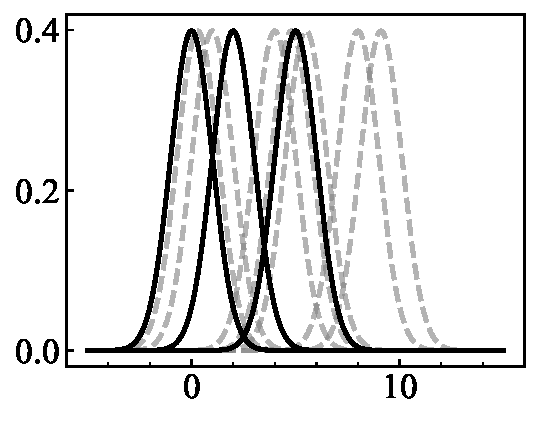
\includegraphics[width=\linewidth]{Figs/FCF_V0}
		\end{subfigure}
		\begin{subfigure}{.18\linewidth}
			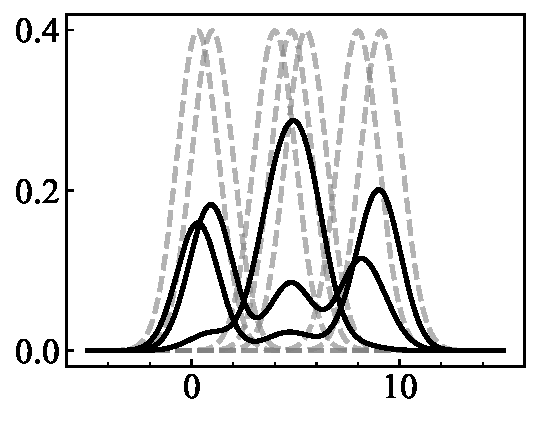
\includegraphics[width=\linewidth]{Figs/FCF_V1}
		\end{subfigure}
		\begin{subfigure}{.18\linewidth}
			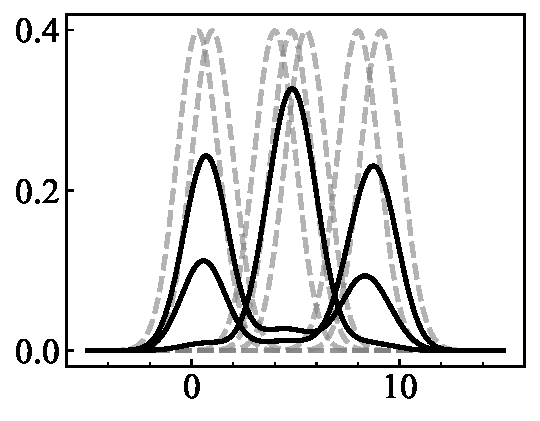
\includegraphics[width=\linewidth]{Figs/FCF_V2}
		\end{subfigure}
		\begin{subfigure}{.18\linewidth}
			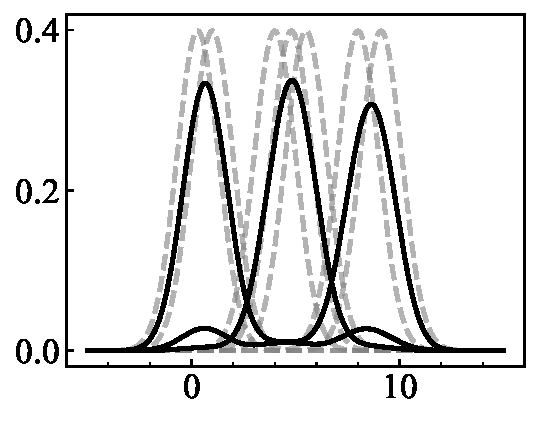
\includegraphics[width=\linewidth]{Figs/FCF_V3}
		\end{subfigure}
		\begin{subfigure}{.18\linewidth}
			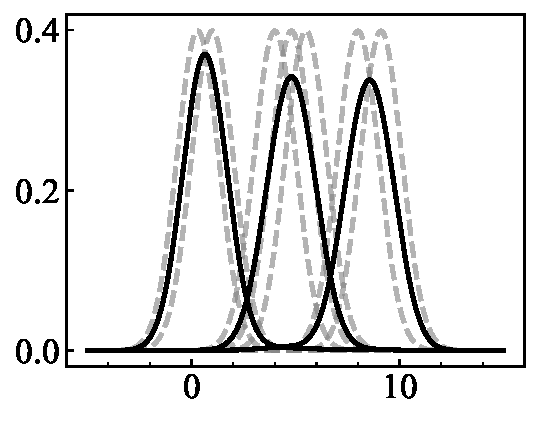
\includegraphics[width=\linewidth]{Figs/FCF_V9}
		\end{subfigure}

	\end{figure}
	
	\begin{figure}[H]
				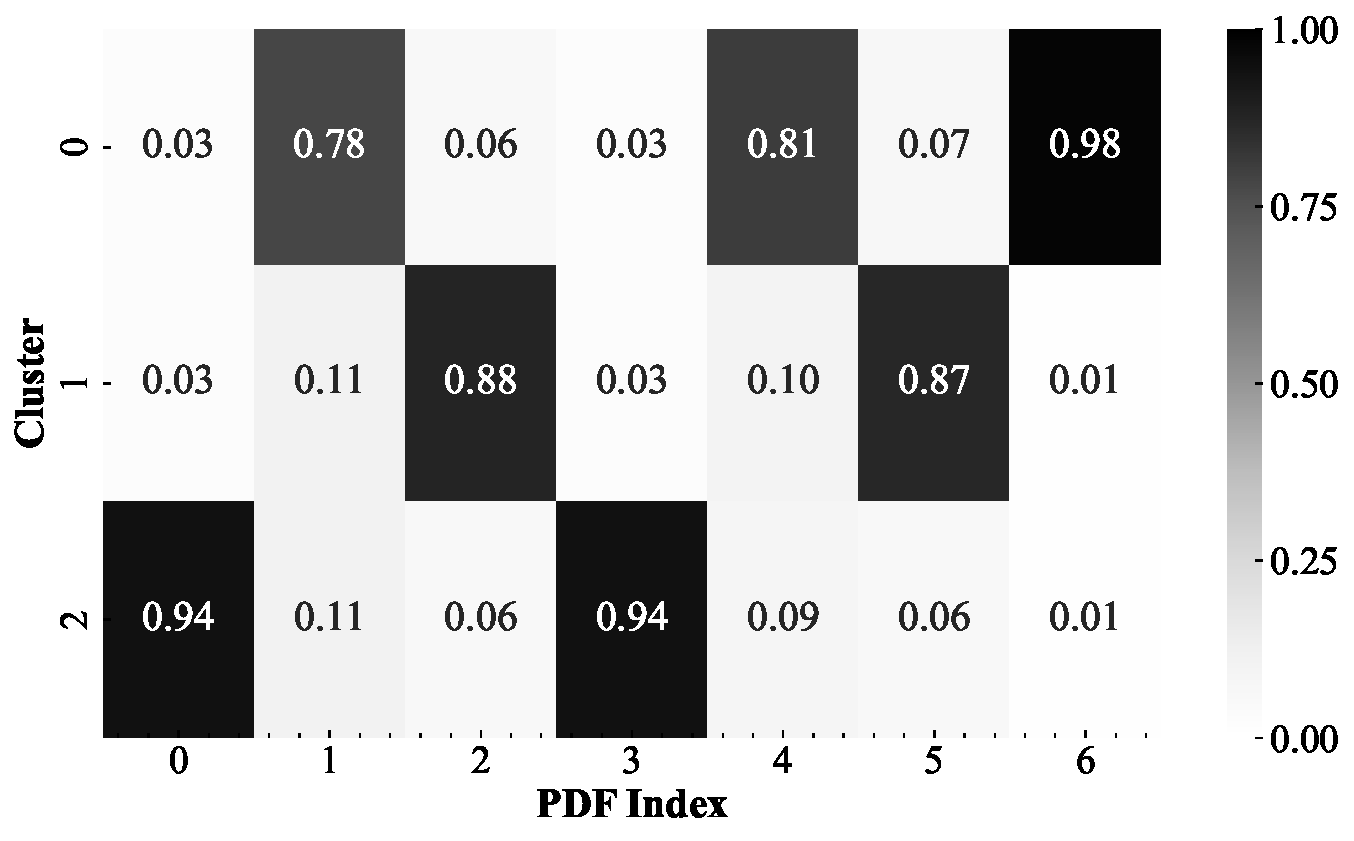
\includegraphics[width=.5\textwidth]{Figs/FCF_U9}
	\end{figure}
\end{frame}


\begin{frame}{1.7. Phân loại hàm mật độ xác suất}{Phương pháp Bayes}
		\begin{figure}
		\centering
		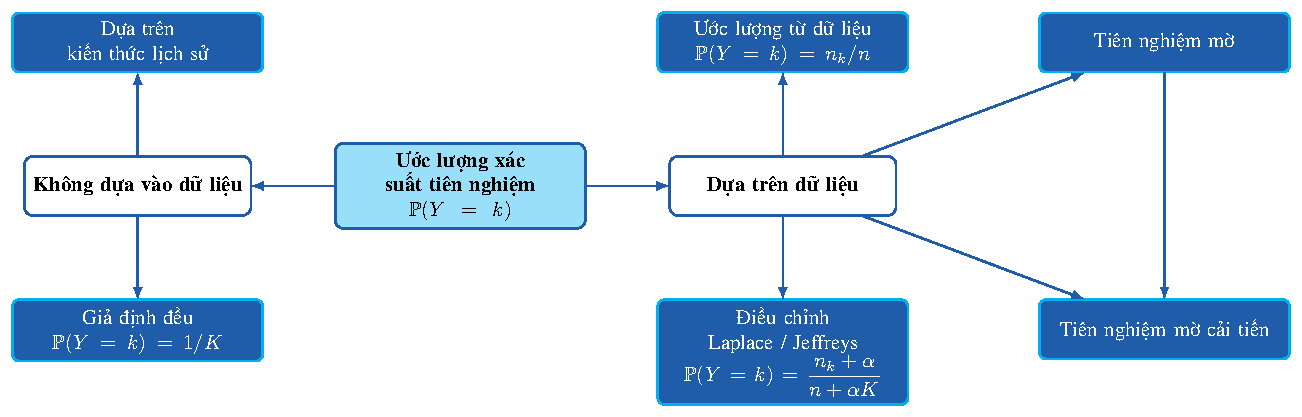
\includegraphics[width=\textwidth]{Figs/bayes1}
	\end{figure}
\end{frame}





\subsection{2. Nhận dạng thống kê mất cân bằng}


\begin{frame}{2.1. Giới thiệu dữ liệu hàm mật độ}

\begin{figure}
	\centering
	\begin{subfigure}{\textwidth}
		\centering
		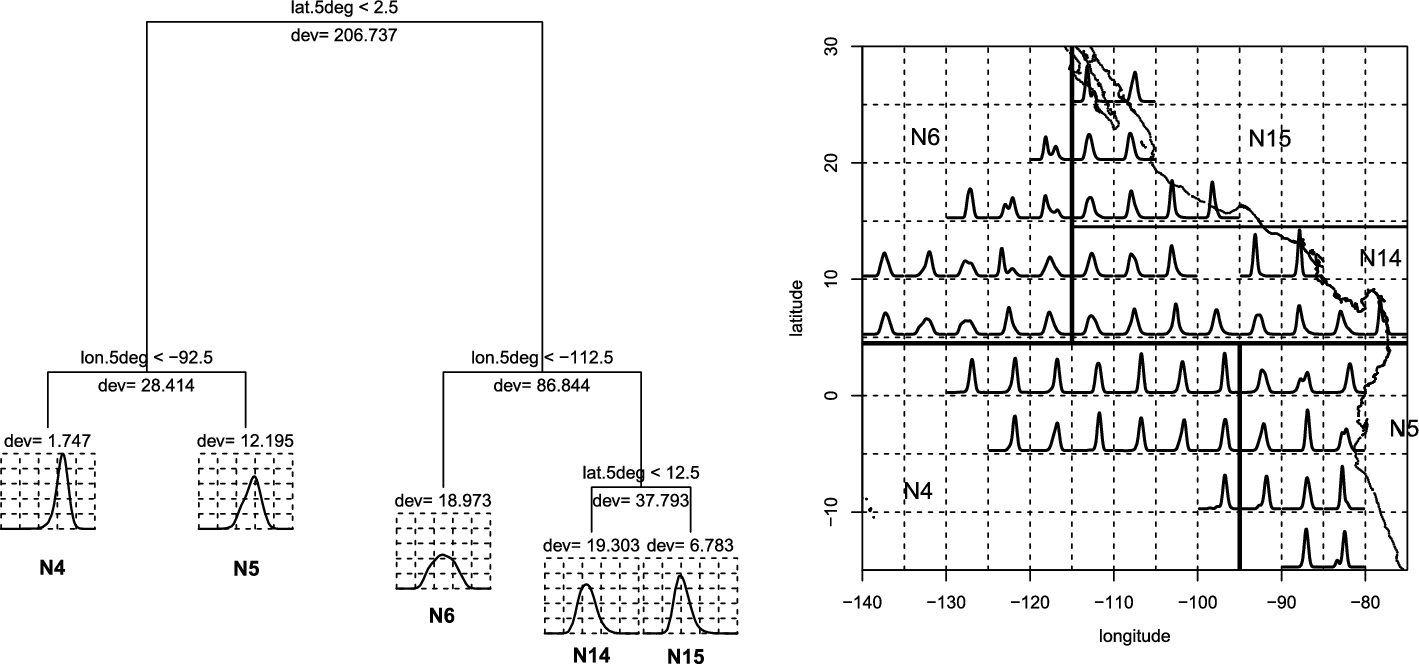
\includegraphics[width=.5\linewidth]{Figs/minami}
	\end{subfigure}\\
	\begin{subfigure}{.32\textwidth}
		\centering
		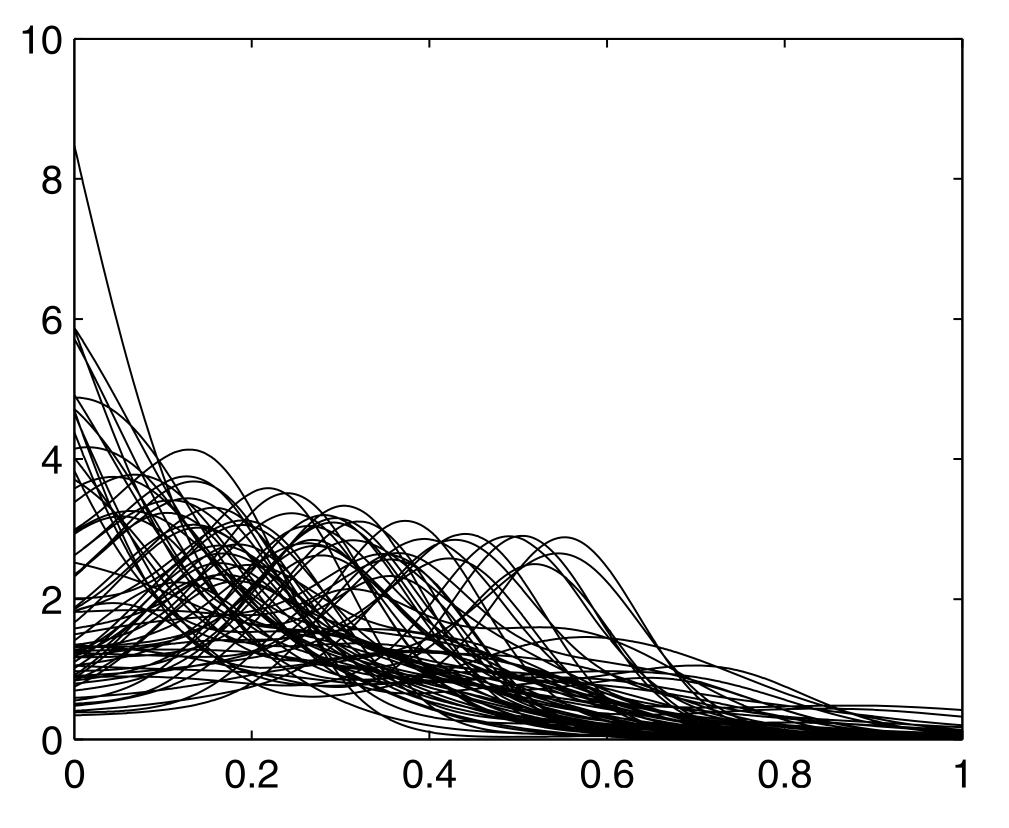
\includegraphics[width=.75\linewidth]{Figs/BOLD}
	\end{subfigure}
	\begin{subfigure}{.32\textwidth}
		\centering
		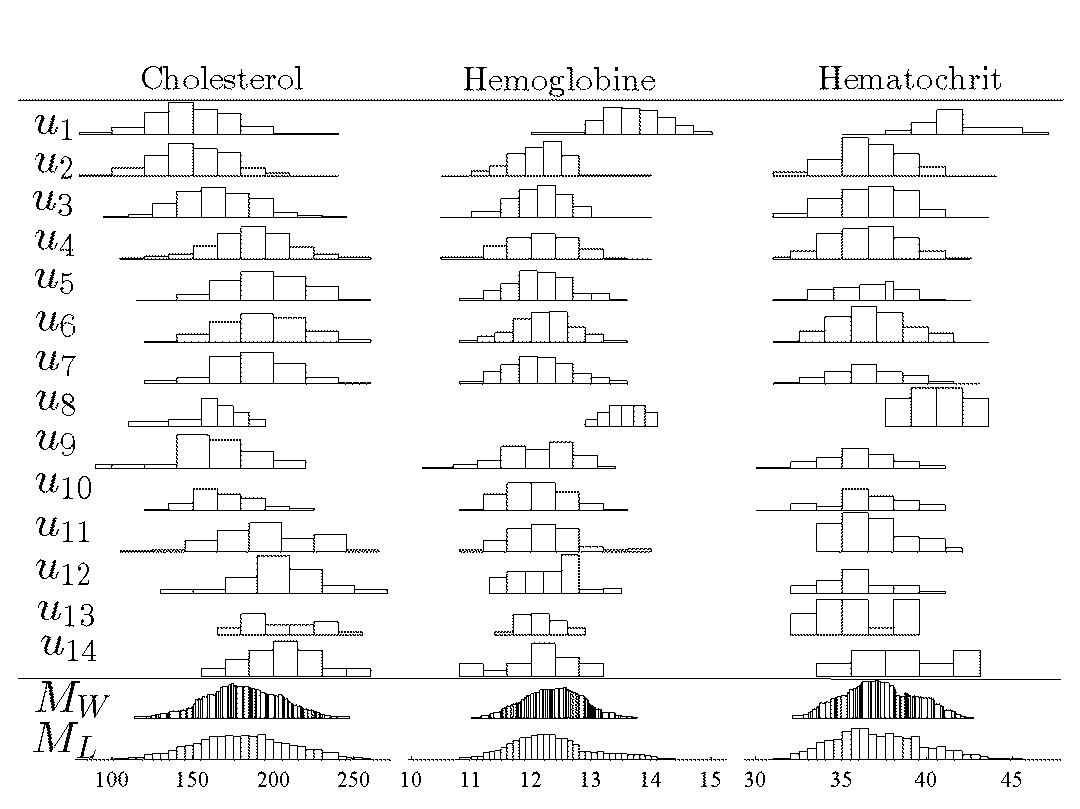
\includegraphics[width=.9\linewidth]{Figs/Blood}
	\end{subfigure}
	\begin{subfigure}{.32\textwidth}
		\centering
		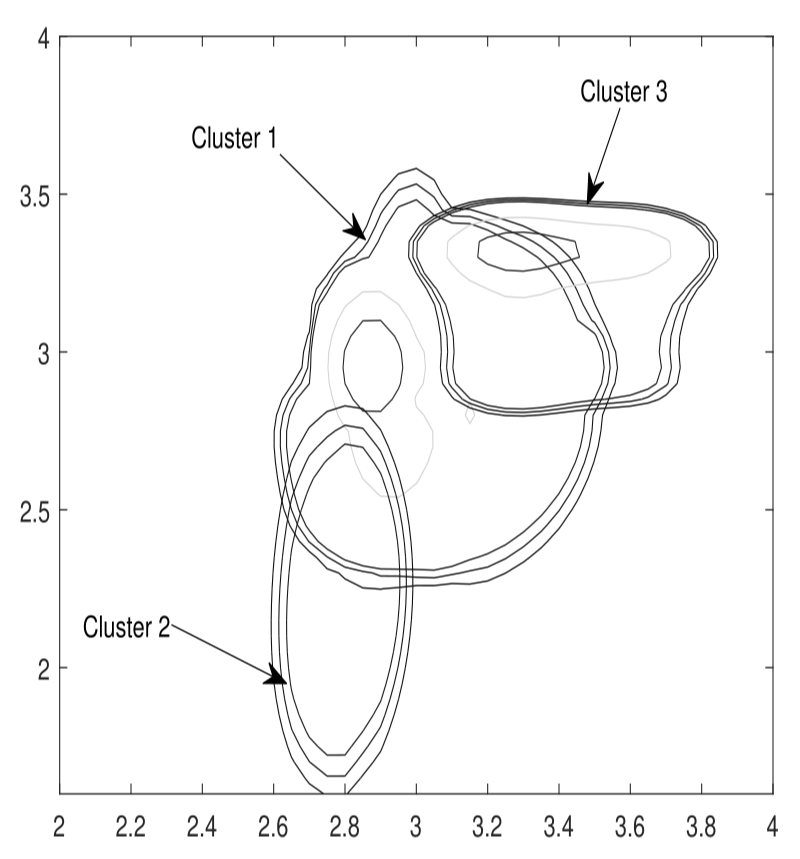
\includegraphics[width=.55\linewidth]{Figs/thao}
	\end{subfigure}
\end{figure}
\end{frame}



\begin{frame}{2.2. Từ FCF đến IFCF}
		\begin{columns}
		\begin{column}{.3\textwidth}
			\begin{figure}
				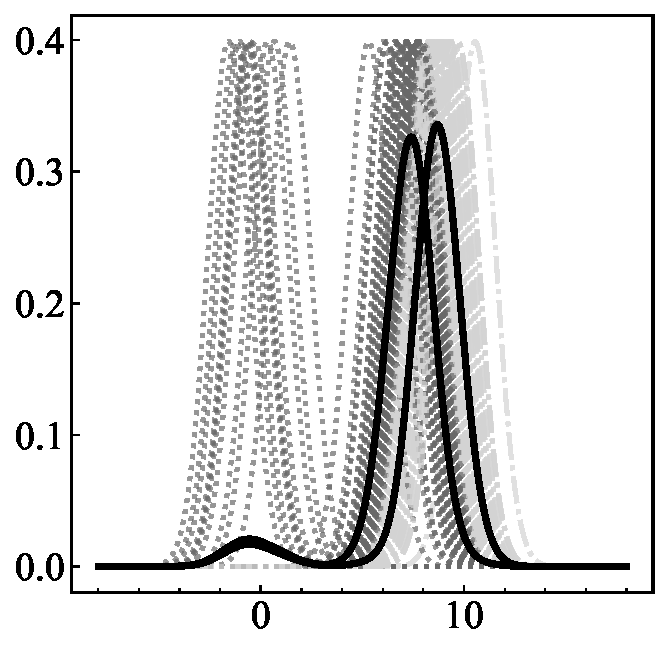
\includegraphics[width=\textwidth]{Figs/FCF_IR10_STD0.8}
			\end{figure}
		\end{column}
		\begin{column}{.6\textwidth}
			Xét hai trọng tâm $\theta_1$ và $\theta_2$ và ma trận phân vùng $\mu_{1j}=u$ và $\mu_{2j}=(1-u)$. Ta có FCF
			\begin{align*}
				\theta_1(x) &= \frac{u^m \sum_{f_j \in c_1} f_j(x) + (1-u)^m \sum_{f_j(x) \in c_2} f_j(x)}{n_1u^m + n_2(1-u)^m},\\
				\theta_2(x) &= \frac{(1-u)^m \sum_{f_j(x) \in c_1} f_j(x) + u^m \sum_{f_j \in c_2} f_j}{n_1(1-u)^m + n_2u^m}.
			\end{align*}
			Giả sử trọng tâm thực tế $\hat\theta_1=\frac1 {n_1}\sum_{f_j \in c_1} f_j(x)$ và $\hat\theta_2=\frac1 {n_2}\sum_{f_j \in c_2} f_j(x)$ thì $\lim\limits_{n_1\to\infty}\mathcal L_2^2=0$.
		\end{column}
	\end{columns}
	
{\color{CTUblue}
			$\Rightarrow$ Cần thiết xây dựng thuật toán phân tích chùm mờ cho mất cân bằng cải tiến vượt qua hiệu ứng đồng nhất.}
	
\end{frame}



\begin{frame}{2.2. Phân tích chùm mất cân bằng (IFCF)}
\begin{block}{Hàm mục tiêu IFCF}
		\begin{align}
		\tag{IFCF}\label{eq:IFCF}
		\text{Minimise}\,&:\, J(\bm U\,;\Theta\,|\, \mathcal{F}\,;c\,;m) = 
		\sum_{j=1}^n \sum_{i=1}^c \frac{1}{\omega_i}\, \mu_{ij}^m \,D^2(f_j\,;\theta_i),\\
		\text{s.t}\,&:\,\sum_{i=1}^{c} \mu_{ij} = 1\,,\quad \forall j \in {1\,,2\,, \ldots\,, n}, \tag{C1}\label{c1_pro} 
	\end{align}
	{\footnotesize	trong đó $\omega_i^{(t)}=\frac{1}{n}\sum_{j=1}^n \mu^{(t-1)}_{ij}$ là tỷ lệ kích thước mờ và $\mu^{(t-1)}_{ij}$ là ma trận phân vùng.}
\end{block}

	
\begin{figure}[H]
	\centering
	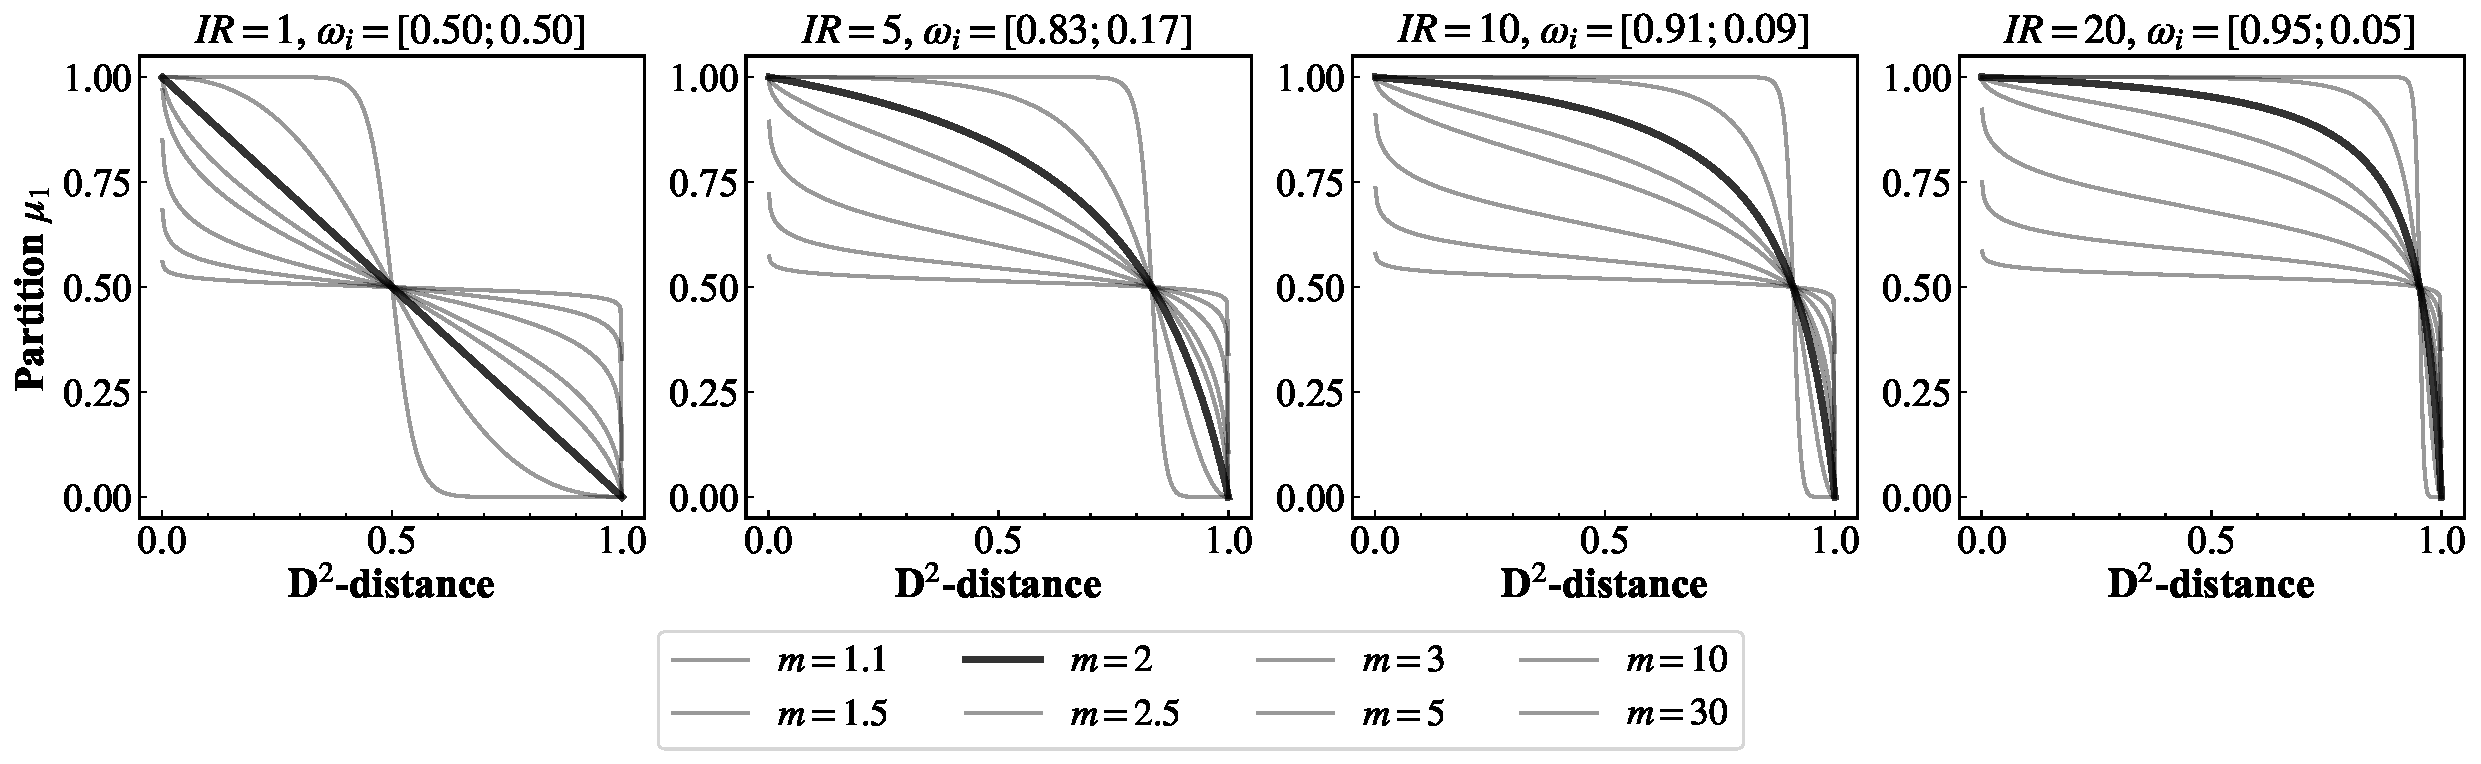
\includegraphics[width=.95\linewidth]{Figs/partition_m.pdf}
\end{figure}
\end{frame}



\begin{frame}{2.2. Phân tích chùm mất cân bằng (IFCF)}
	\begin{columns}
		\begin{column}{.5\textwidth}
			\small
			\begin{lemma}[Cập nhật ma trận phân vùng $\bm U$]\label{lem1}
				Với $\Theta$ cố định, bài toán tối ưu hoá $J_{IFCF}$ theo $\bm U$ có nghiệm cực tiểu duy nhất $\bm U^*=F(\Theta)$ dưới các ràng buộc phân hoạch mờ \eqref{c1_pro}. Cụ thể,
				\begin{align}
					\mu_{ij} \;=\;
					\frac{
						\left (\frac{\omega_i}{\,D^2(\theta_i\,;f_j)}\right)^{\frac{1}{m-1}}
					}{
						\sum_{s=1}^c
						\left(\frac{\omega_s}{\,D^2(\theta_s\,;f_j)}\right)^{\frac{1}{m-1}}
					},
					\label{eq:ifcf_u_final}
				\end{align}
				trong đó $1\le i\le c$ và $1\le j\le n$.
			\end{lemma}
			Ngoài ra, nếu $\exists i_0$ sao cho $D^2(\theta_{i_0}\,;f_j)=0$ thì nghiệm tối ưu cho cột $j$ là $\mu_{i_0 j}=1$ và $\mu_{s j}=0$, $\forall s\neq i_0$.
		\end{column}
		\begin{column}{.5\textwidth}
			\small
			\begin{lemma}[Cập nhật trọng tâm $\Theta$ với $\mathcal{L}_2^2$]\label{lem2}
				Với $\bm U$ cố định, bài toán tối thiểu hoá $J_{IFCF}$ theo $\Theta$ là phân tích được theo từng $\theta_i$ với $i =1\,,2\,,\ldots\,,c$ và lồi nghiêm ngặt. Tồn tại duy nhất nghiệm cực tiểu $\Theta^*=G(\bm U)$ khi khoảng cách $D^2=\mathcal{L}_2^2$, 
				\begin{align}
					\theta_i(x)
					\;=\;
					\frac{\sum_{j=1}^n (\mu_{ij})^{m}\,f_j(x)}
					{\sum_{j=1}^n (\mu_{ij})^{m}}.
					\label{eq:theta_update}
				\end{align}
			\end{lemma}
		\end{column}
	\end{columns}
	{\color{CTUblue}
		$\Rightarrow$ Thuật toán hội tụ qua các vòng lặp đối với $\mathcal{L}_2$ và $D_H^2$ (Định lý Zangwill).
		}
\end{frame}


\begin{frame}{2.3. Phân tích chùm mất cân bằng (IFCF)}{Ví dụ số}
		Giả sử dữ liệu được tạo theo công thức tổng quát về kỳ vọng và độ lệch chuẩn của mỗi chùm, cụ thể như sau:
	\begin{align*}
		\begin{array}{clll}
			\text{Chùm } 1: & f(x\,\vert \,\mu\,;\sigma^2)\sim \mathcal{N}(\mu_1\,;\sigma_1^2)\,; 
			\text{với } \mu_1 \sim \mathcal{N}(-5{,}0\,;1{,}0)\,;\;\sigma_1 = 2{,}0,\\
			\text{Chùm } 2: & f(x\,\vert \,\mu\,;\sigma^2)\sim \mathcal{N}(\mu_2\,;\sigma_2^2)\,; 
			\text{với } \mu_2 \sim \mathcal{N}(5{,}0\,;1{,}0)\,;\;\sigma_2 = 4{,}0.
		\end{array}
	\end{align*}

	
	\begin{figure}[H]
		\centering
		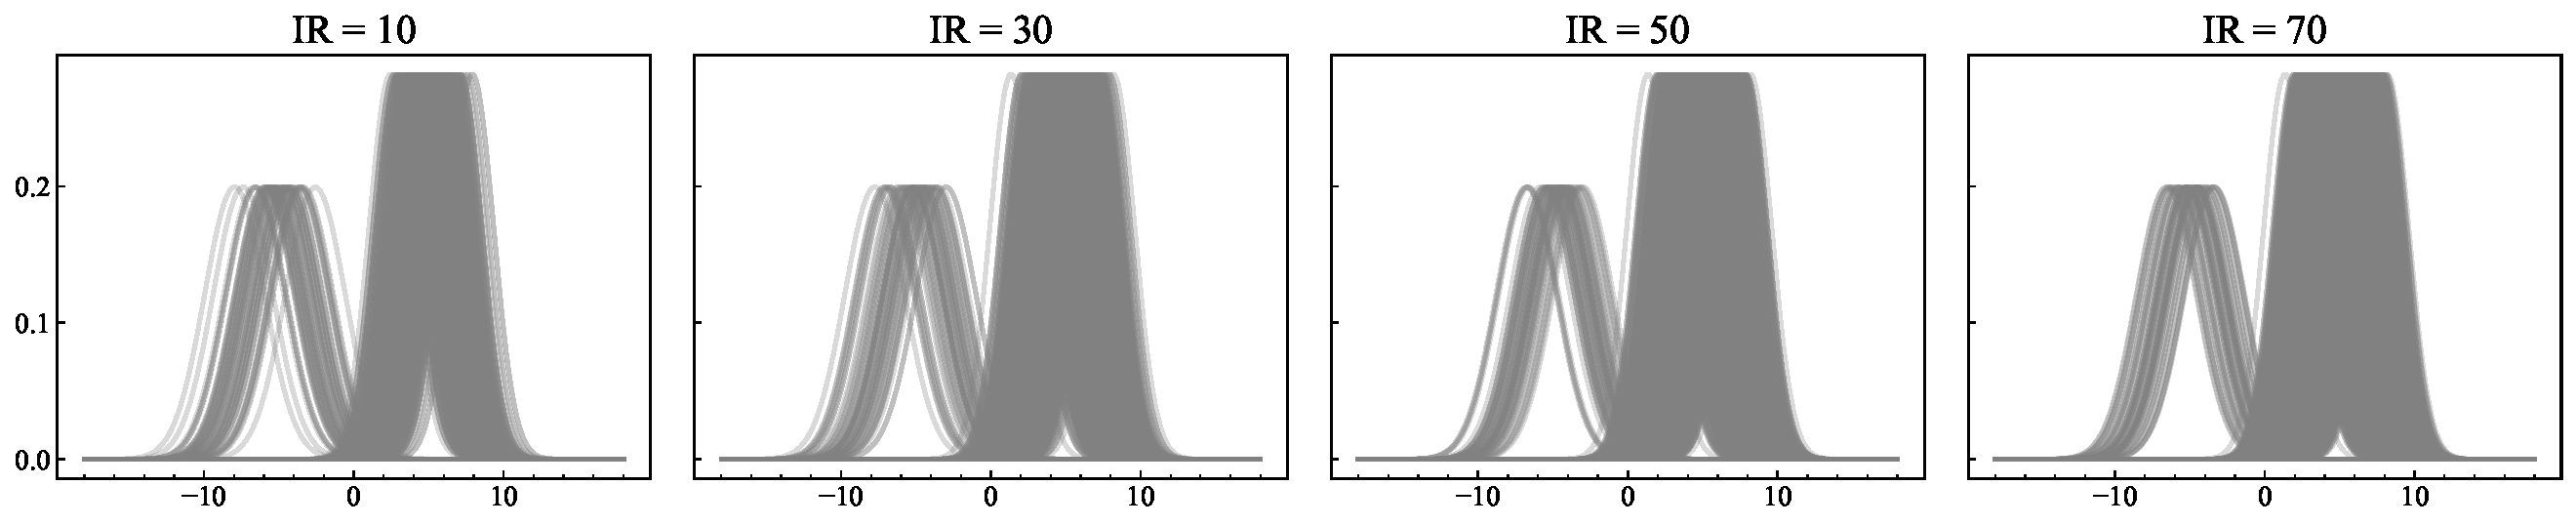
\includegraphics[width=\linewidth]{Figs/pdf_bandau}
	\end{figure}
\end{frame}

\begin{frame}{2.3. Phân tích chùm mất cân bằng (IFCF)}{Kết quả các loại khoảng cách}
	
	\begin{figure}[H]
		\centering
		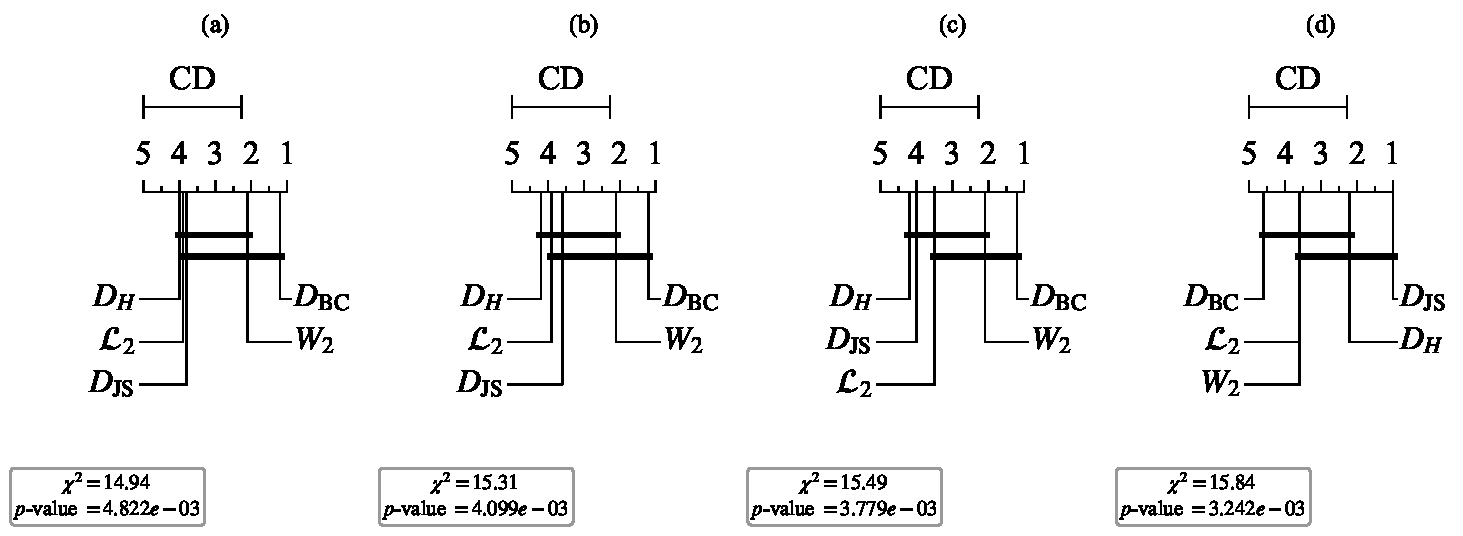
\includegraphics[width=\linewidth]{Figs/eva_distances}	
\begin{flushleft}\footnotesize
	Chú thích: (a) ARI, (b) NMI, (c) $Silhouette$ và (d) thời gian tính toán.
\end{flushleft}
	\end{figure}
\end{frame}


\begin{frame}{2.3. Phân tích chùm mất cân bằng (IFCF)}{ Kết quả các tham số mờ}
	
	\begin{figure}[H]
		\centering
		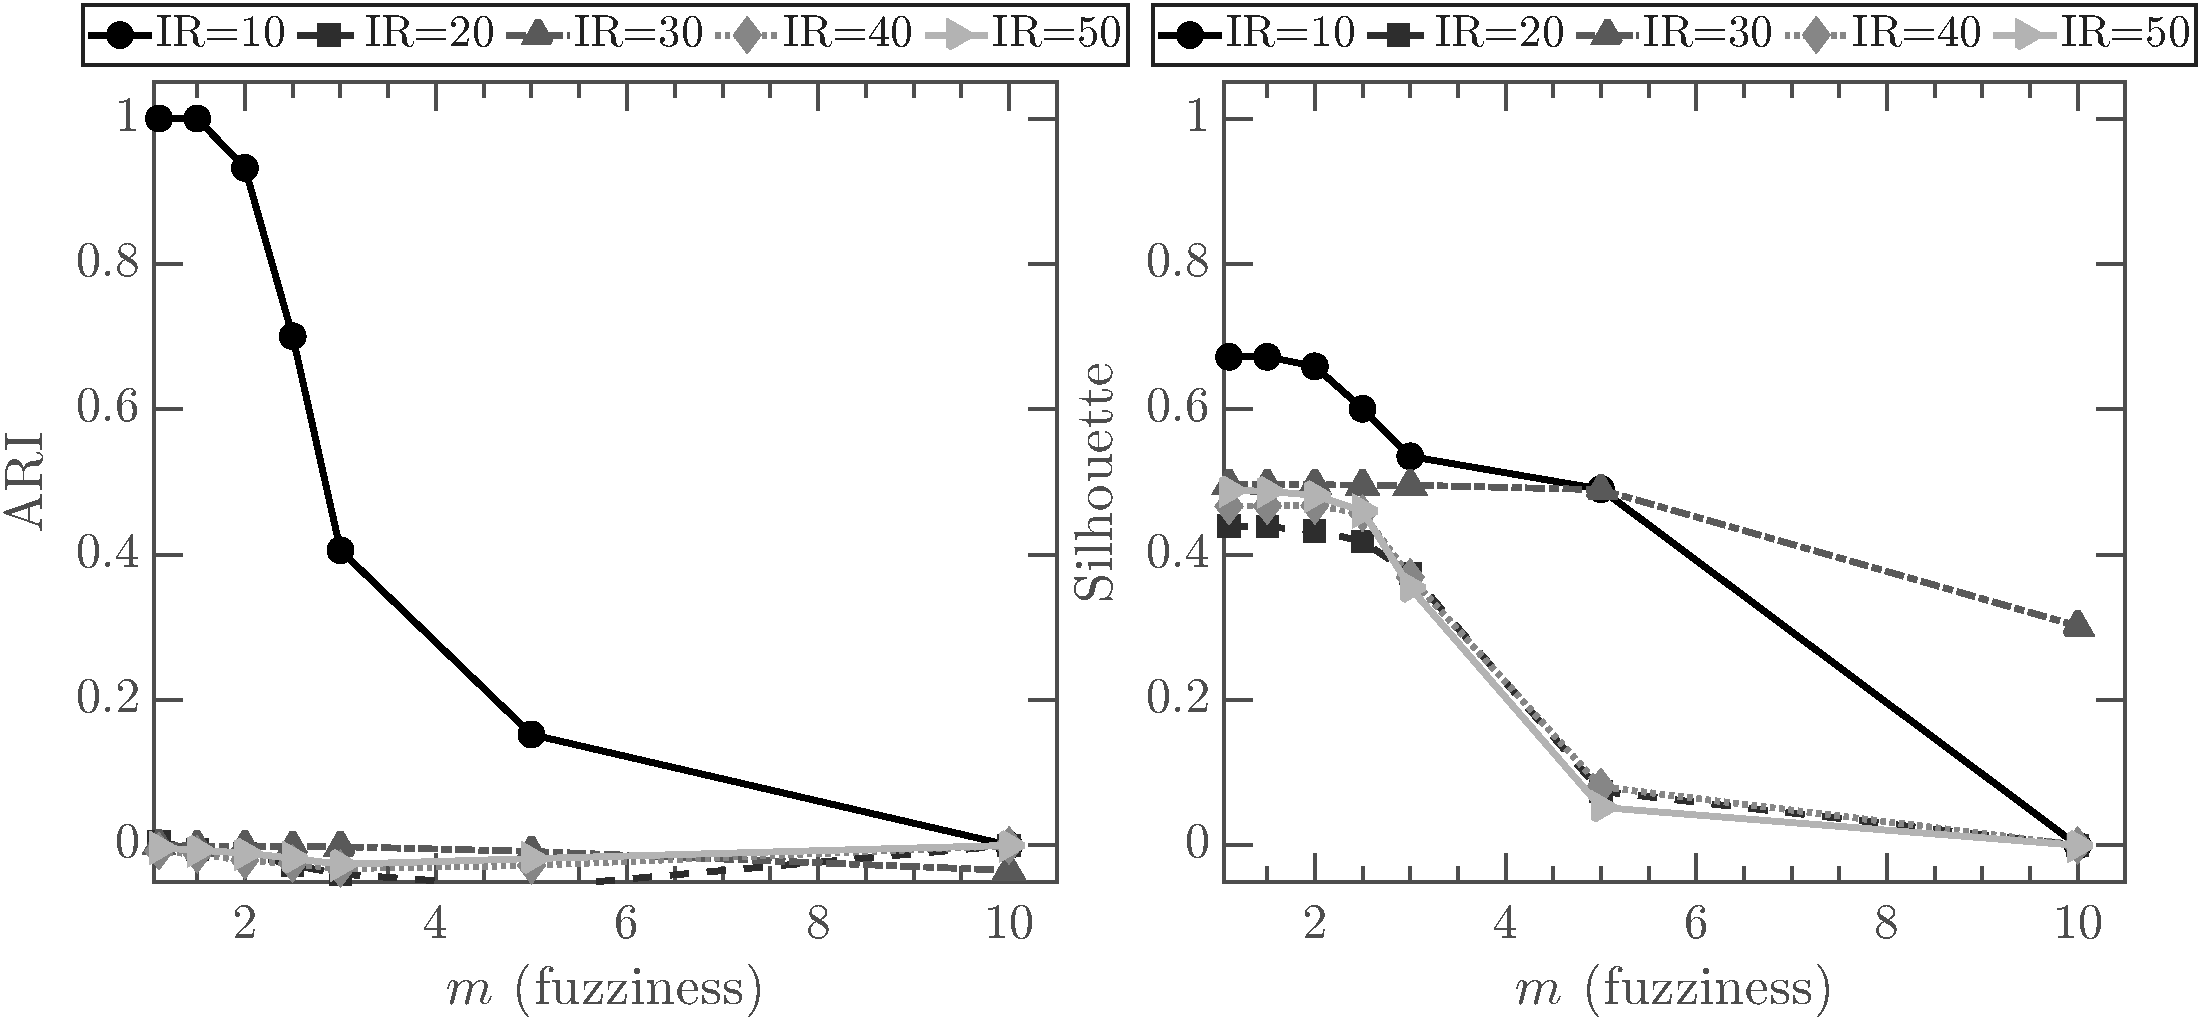
\includegraphics[width=.7\linewidth]{Figs/figM}
	\end{figure}
	\begin{flushleft}\footnotesize
	Chú thích:	$m=\{1.1\,,1.5\,,2.0\,,2.5\,,3.0\,,5.0\,,10.0\}$
	\end{flushleft}
\end{frame}

\begin{frame}{2.3. Phân tích chùm mất cân bằng (IFCF)}{ Kết quả thuật toán phân tích chùm}
	\begin{figure}[H]
		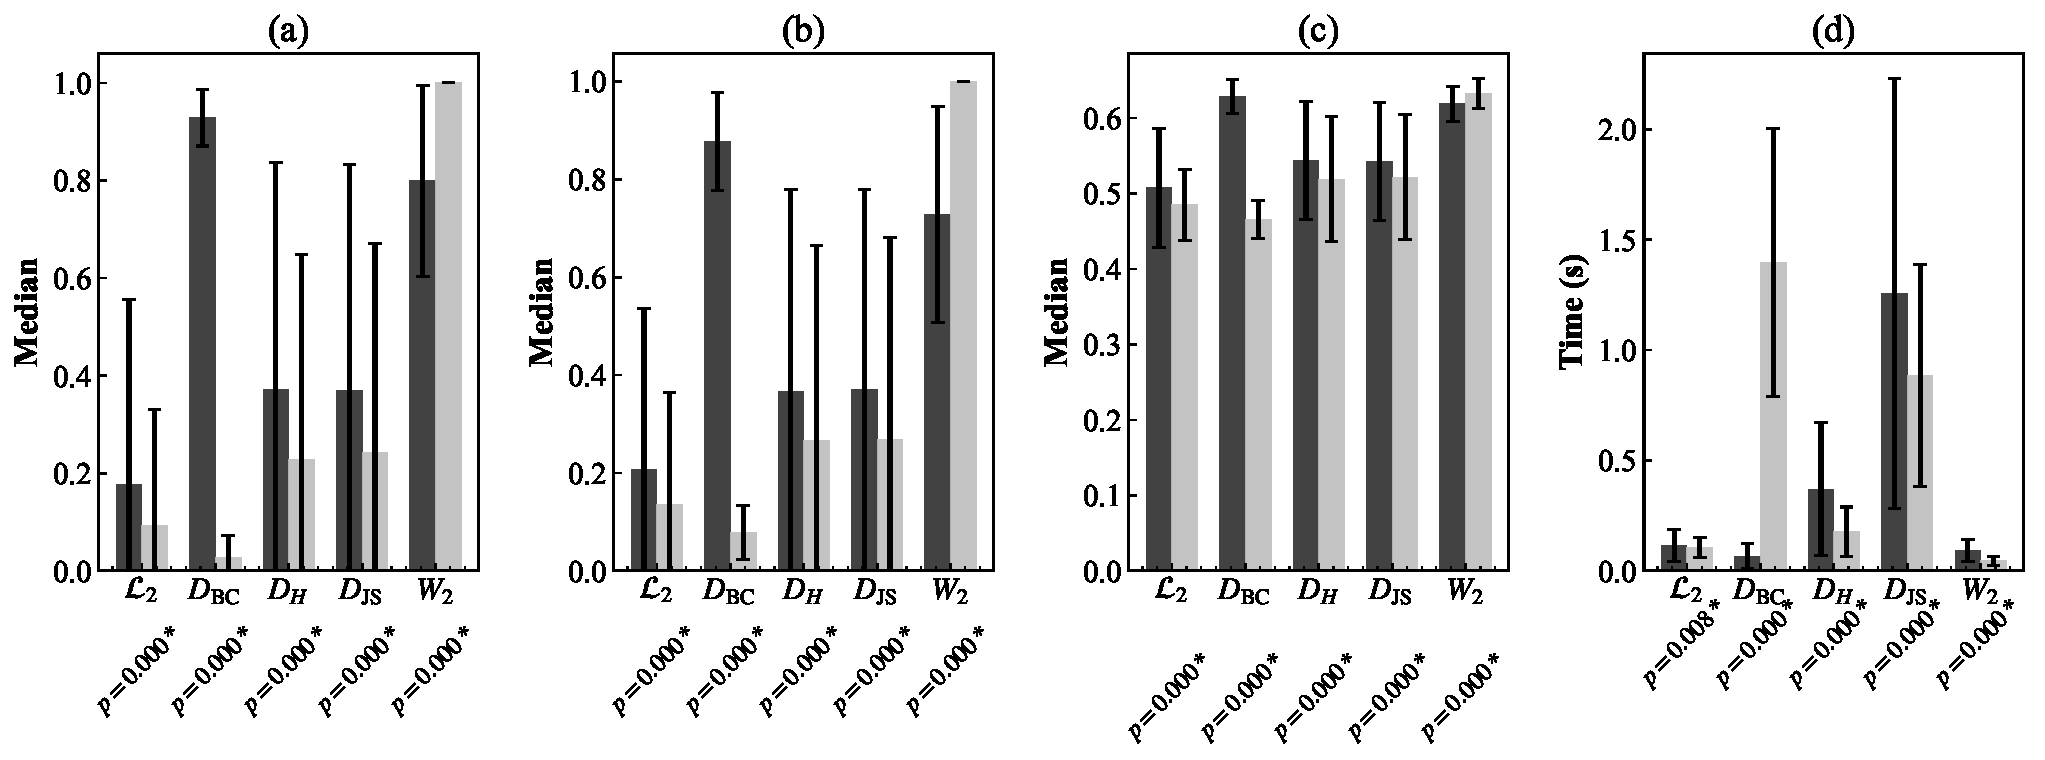
\includegraphics[width=\linewidth]{Figs/eva_by_distance_wilcoxon}
	\end{figure}
	\begin{flushleft}\footnotesize
		Chú thích: (a) ARI, (b) NMI, (c) $Silhouette$ và (d) thời gian tính toán.
	\end{flushleft}
\end{frame}




\begin{frame}{2.4. Phân loại mất cân bằng (Bayes-IFCF)}
\begin{columns}
	\begin{column}{.6\textwidth}
		\begin{figure}[H]
			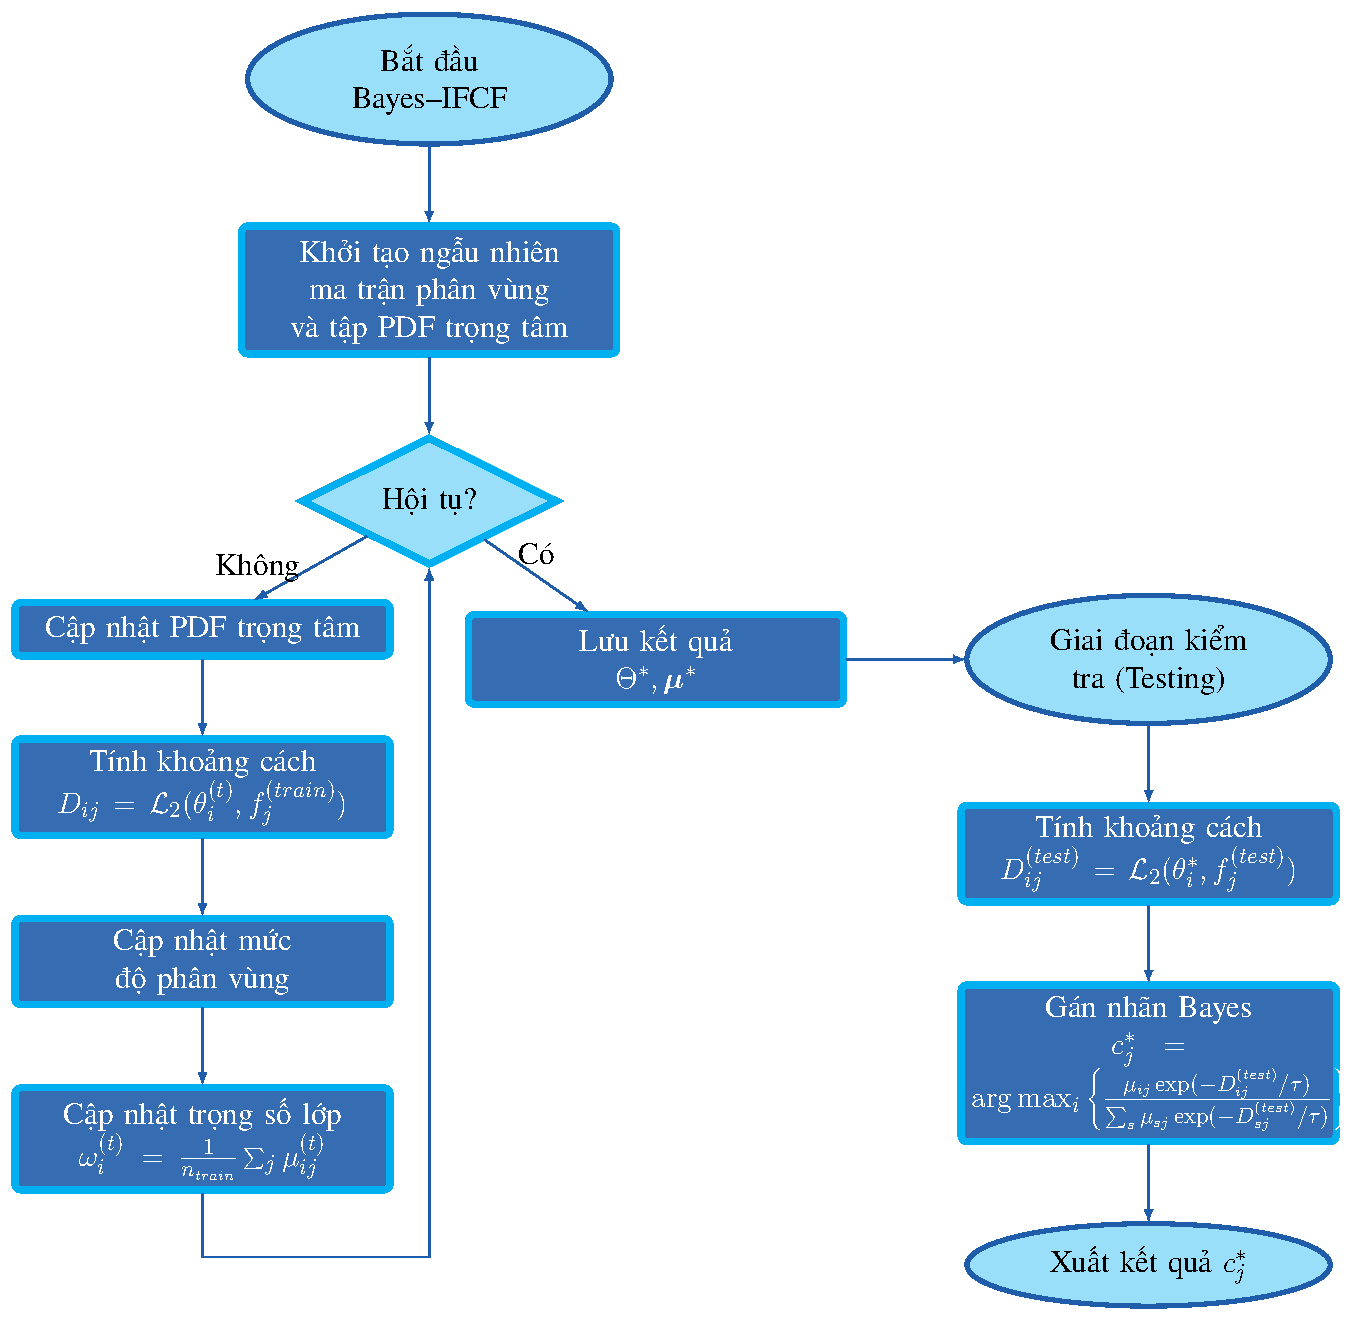
\includegraphics[width=.9\linewidth]{Figs/bayes2}
		\end{figure}
	\end{column}
	\begin{column}{.4\textwidth}\footnotesize
		Quy tắc Bayes cải tiến, xếp một PDF mới vào lớp $c_i$ nếu $$c_i = \arg\max_{i}\left\{\frac{\bm U^{(test)}_{ij} \exp\left (-\bm D^{(test)}_{ij}/\tau\right )}{\displaystyle\sum_s\bm U^{(test)}_{sj} \exp\left (-\bm D^{(test)}_{sj}/\tau\right )}\right\},$$ trong đó khoảng cách $D$ được chuẩn hóa với $\tau=\frac{1}{n_{test}}\sum_iD_{ij}$ . 
		
		Nguyên tắc này chỉ định rằng một PDF được gán vào một lớp cụ thể nếu nó đồng thời sở hữu giá trị cao nhất đối với xác suất tiên nghiệm và độ đo tương đồng đối với lớp đó.
	\end{column}
\end{columns}
\end{frame}

\begin{frame}{2.5. Phân loại mất cân bằng (Bayes-IFCF)}{Ví dụ số}
	
	\begin{figure}[H]
		\begin{subfigure}{.5\textwidth}
			\centering
			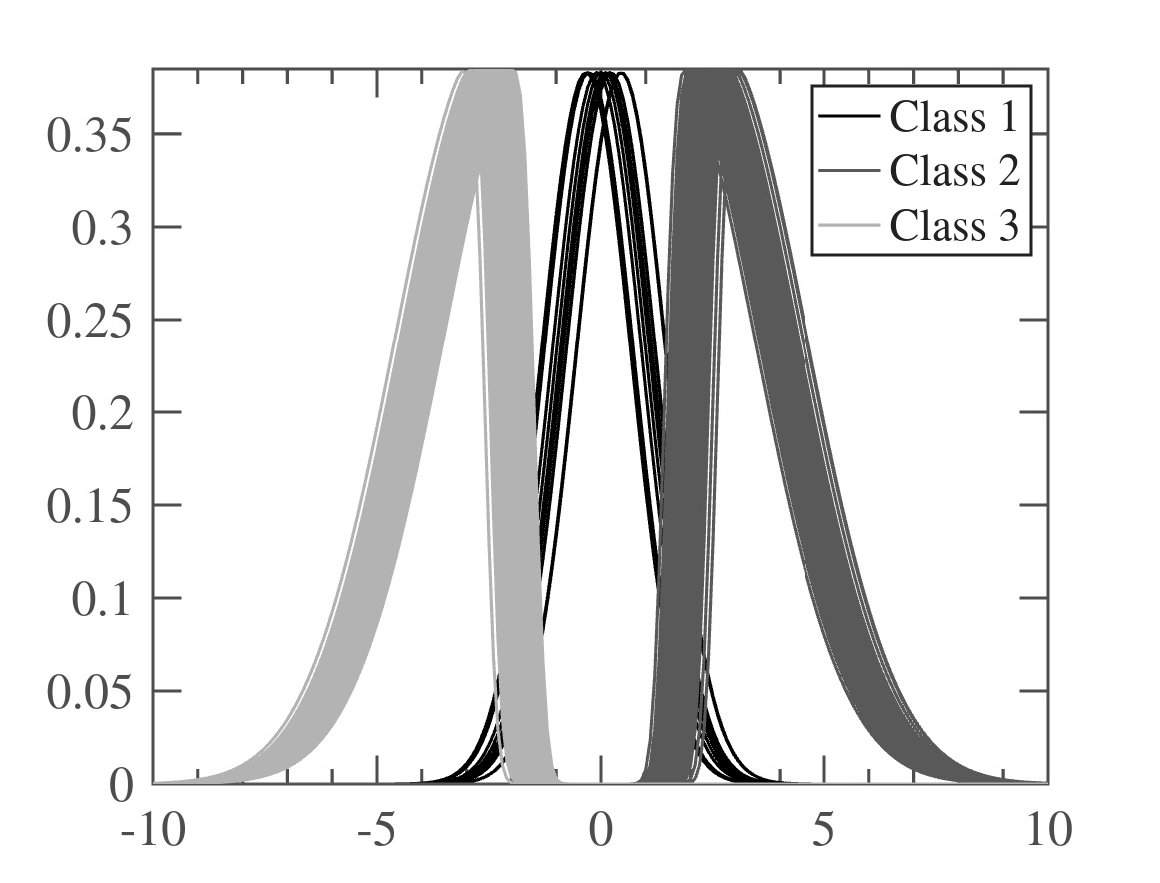
\includegraphics[width=.45\linewidth]{Figs/vidu2_full}
			\caption{$10:200:200$}
		\end{subfigure}
		\begin{subfigure}{.45\textwidth}
			\centering
			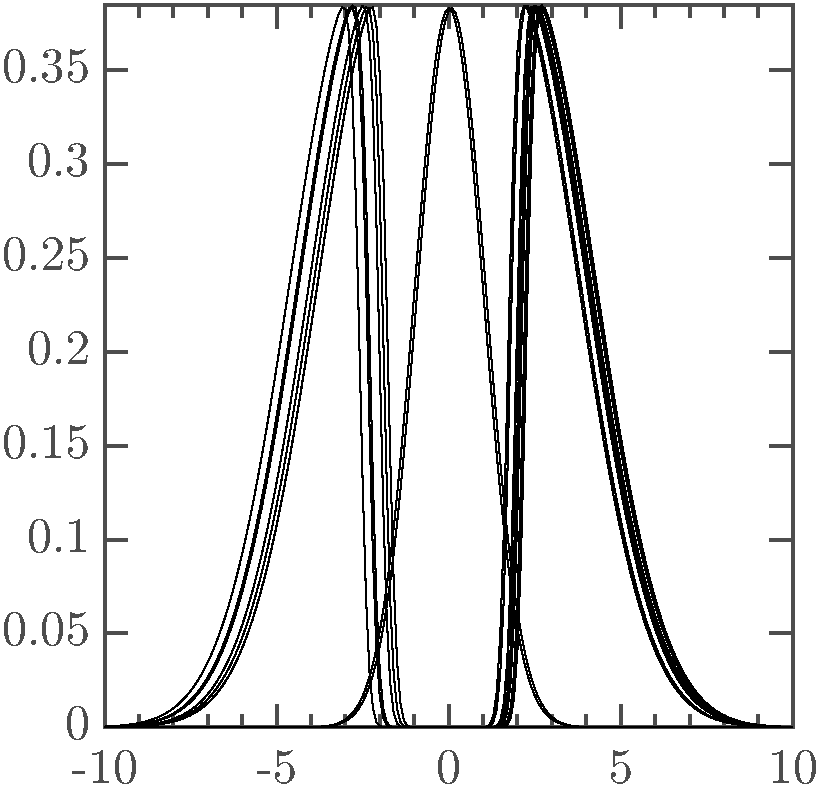
\includegraphics[width=.4\linewidth]{Figs/vidu2_test}
			\caption{$2:10:8$}
		\end{subfigure}
	\end{figure}
	
	\begin{figure}[H]
		\centering
		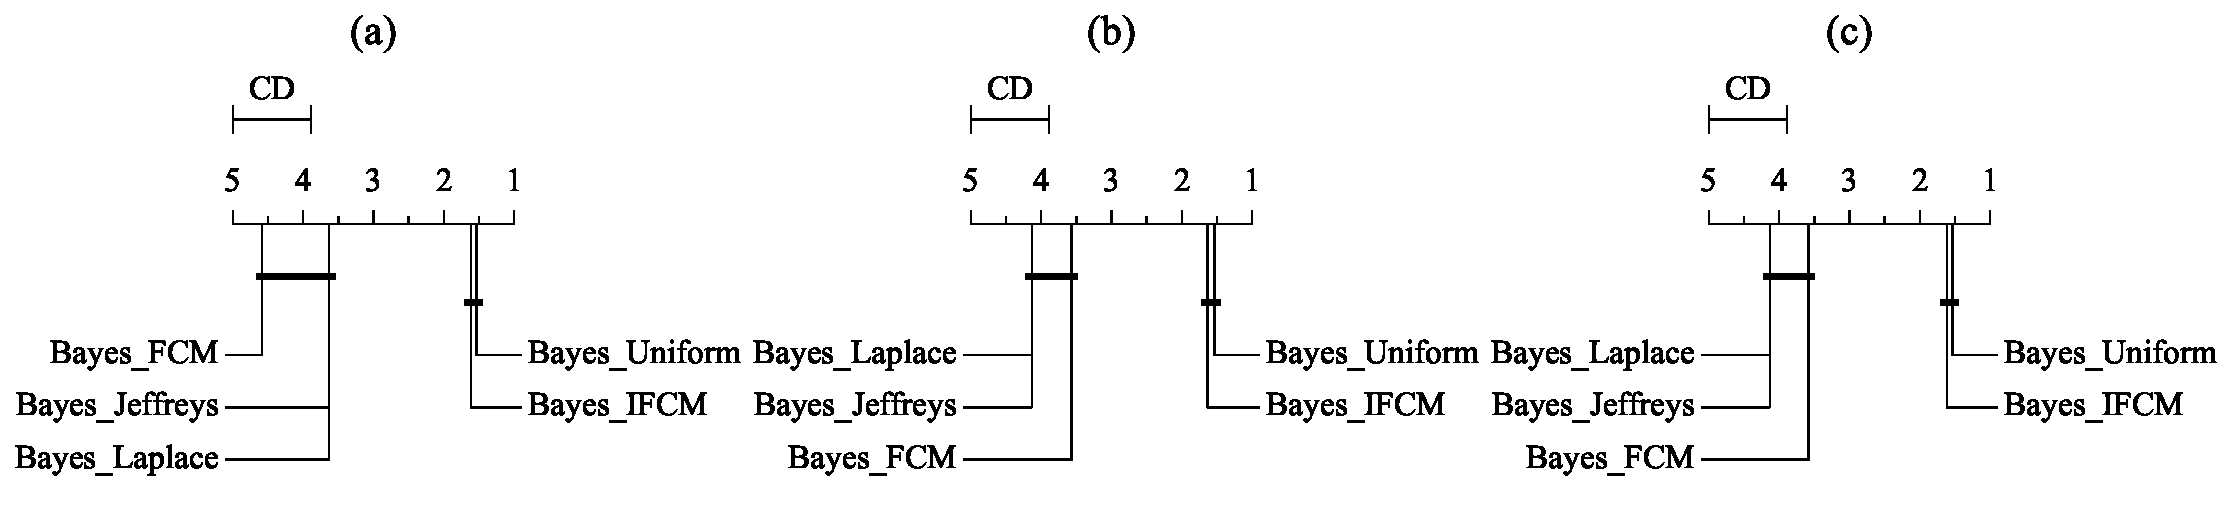
\includegraphics[width=\linewidth]{Figs/CD_3metrics}
		\begin{flushleft}\footnotesize
			Chú thích: (a) ACC, (b) F1-score, (d) thời gian tính toán.
		\end{flushleft}
	\end{figure}
	
\end{frame}



\subsection{3. Ứng dụng cho dữ liệu hình ảnh}

\begin{frame}{3.1. Vấn đề trích xuất đặc trưng hình ảnh}{Ước lượng màu sắc vs ước lượng khối màu}
	\begin{columns}
		\begin{column}{.5\textwidth}
			\begin{figure}
				\centering
				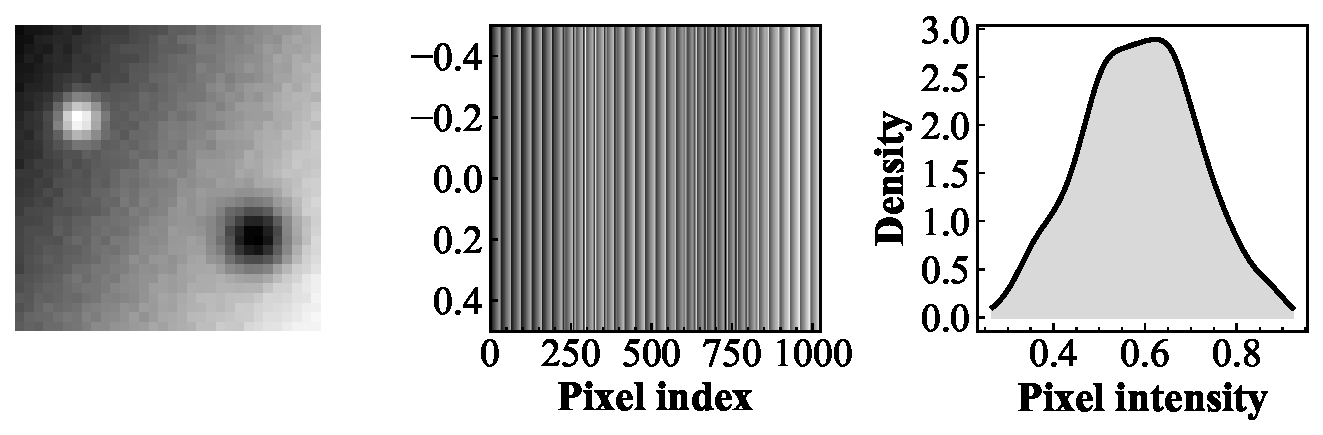
\includegraphics[width=.8\linewidth]{Figs/kde_image_density}
				\caption{Ước lượng màu sắc}
			\end{figure}
		\end{column}
		\begin{column}{.5\textwidth}
			\begin{figure}
				\centering
				
\includegraphics[width=.5\linewidth]{Figs/kde_patches_density}
				\caption{Ước lượng khối màu}
			\end{figure}
		\end{column}
	\end{columns}
\end{frame}



\begin{frame}{3.2. Phân tích chùm mất cân bằng (IFCF)}{Ví dụ hình ảnh dựa vào ước lượng màu sắc}
	\begin{columns}
		\begin{column}{.5\textwidth}
			
			\begin{figure}
				\centering
				\begin{subfigure}[b]{.4\linewidth}
					\centering
					
\includegraphics[width=\textwidth]{Figs/D82.png}
					\caption{}
				\end{subfigure}
				\begin{subfigure}[b]{.4\linewidth}
					\centering
					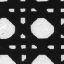
\includegraphics[width=\textwidth]{Figs/D102.png}
					\caption{}
				\end{subfigure}\hfill\\
				\begin{subfigure}[b]{.3\linewidth}
					\centering
					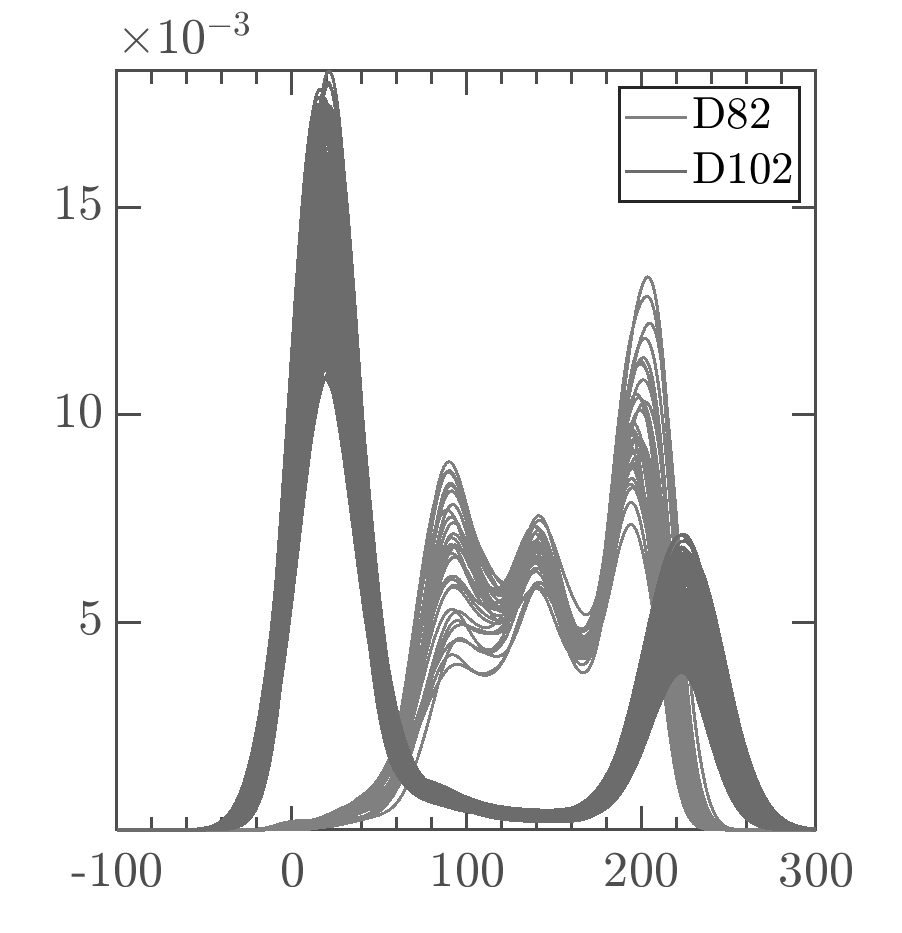
\includegraphics[width=\textwidth]{Figs/EX2_IR_10}
					\caption{}
				\end{subfigure}
				\begin{subfigure}[b]{.3\linewidth}
					\centering
					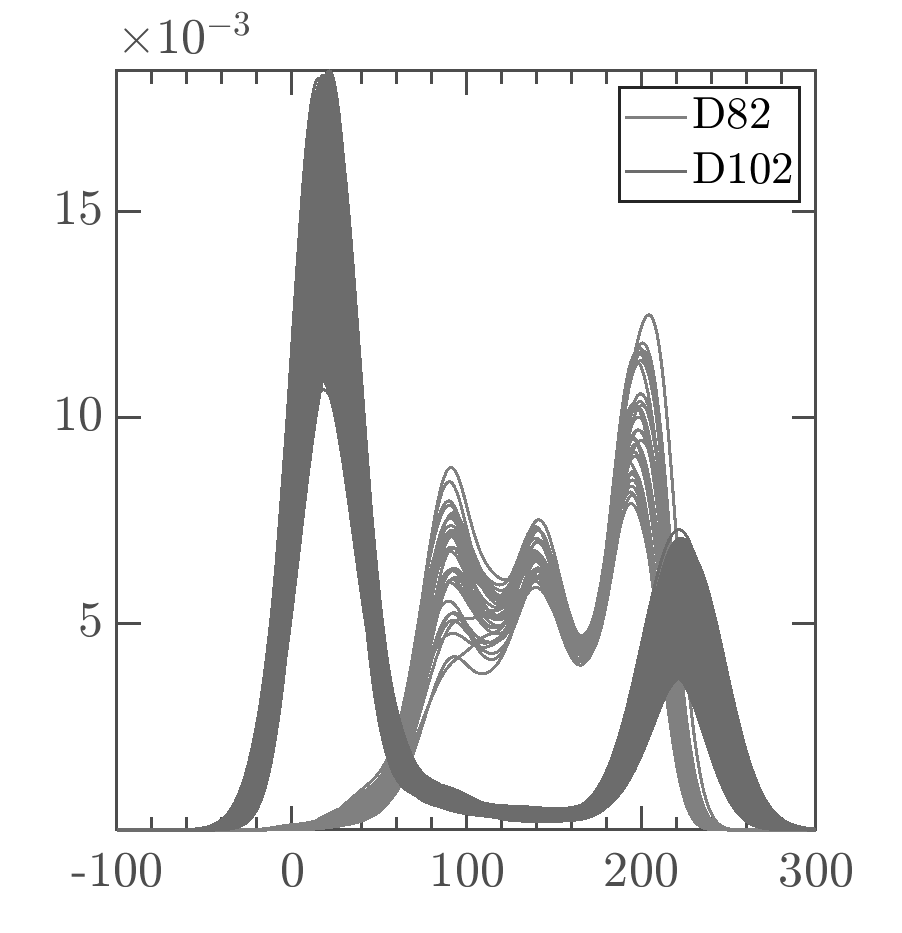
\includegraphics[width=\textwidth]{Figs/EX2_IR_50}
					\caption{}
				\end{subfigure}
				\begin{subfigure}[b]{.3\linewidth}
					\centering
					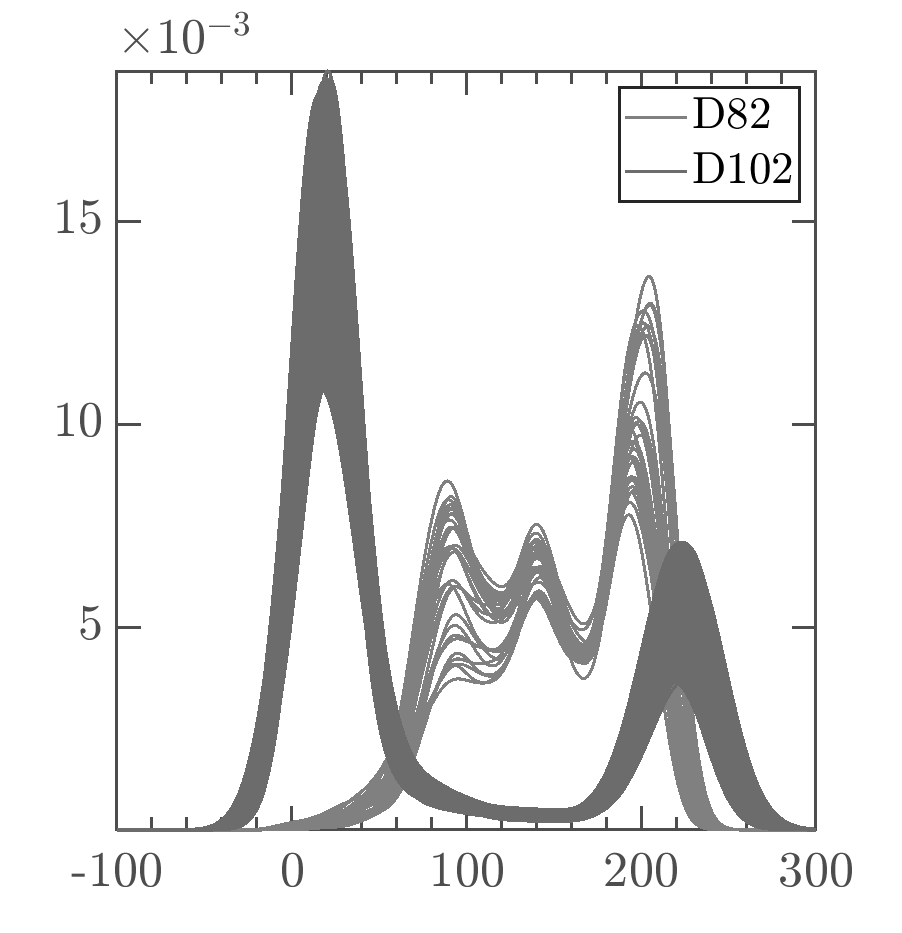
\includegraphics[width=\textwidth]{Figs/EX2_IR_100}
					\caption{}
				\end{subfigure}
			\end{figure}
		\end{column}
		\begin{column}{.5\textwidth}
			\begin{figure}
				\centering
				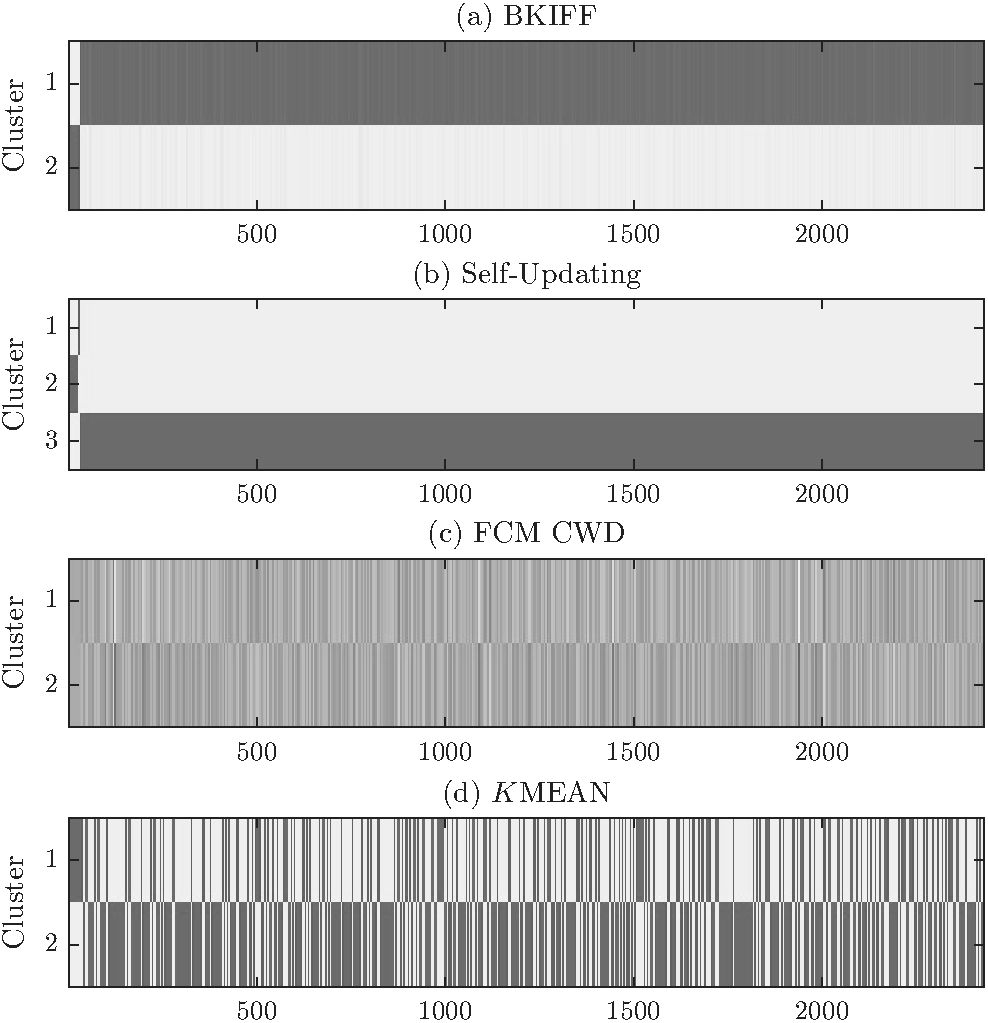
\includegraphics[width=\linewidth]{Figs/fig:U_ex3.pdf}
			\end{figure}
		\end{column}
	\end{columns}
\end{frame}



\begin{frame}{3.2. Phân tích chùm mất cân bằng (IFCF)}{Ví dụ hình ảnh dựa vào ước lượng màu sắc}

		\begin{figure}
			\centering
			\begin{subfigure}[h]{0.32\linewidth}
				\centering
				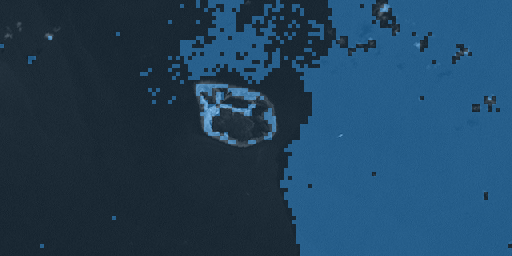
\includegraphics[width=.8\linewidth]{Figs/BKIFF_k2}
				\caption{$c=2$}
			\end{subfigure}
			\begin{subfigure}[h]{0.32\linewidth}
				\centering
				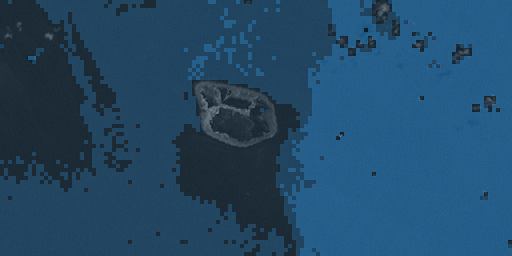
\includegraphics[width=.8\linewidth]{Figs/BKIFF_k3}
				\caption{$c=3$}
			\end{subfigure}
			\begin{subfigure}[h]{0.32\linewidth}
				\centering
				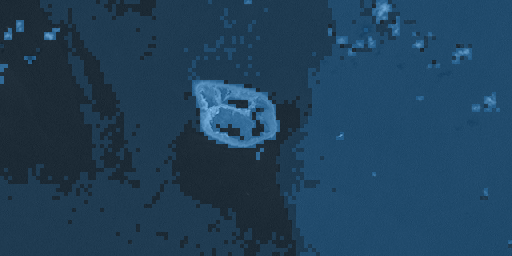
\includegraphics[width=.8\linewidth]{Figs/BKIFF_k4}
				\caption{$c=4$}
			\end{subfigure}\hfil\\
			\begin{subfigure}[h]{0.32\linewidth}
				\centering
				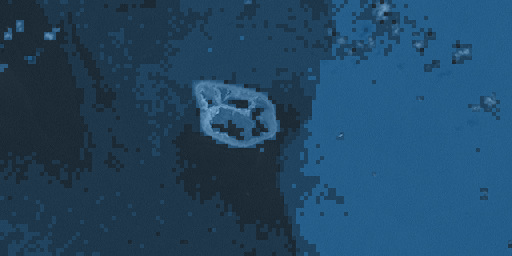
\includegraphics[width=.8\linewidth]{Figs/BKIFF_k5}
				\caption{$c=5$}
			\end{subfigure}
			\begin{subfigure}[h]{0.32\linewidth}
				\centering
				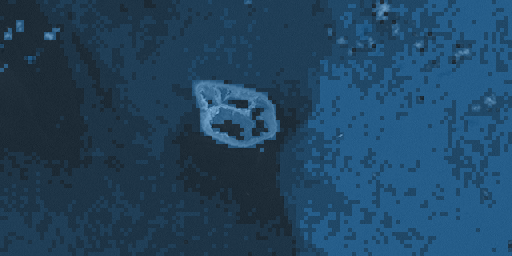
\includegraphics[width=.8\linewidth]{Figs/BKIFF_k6}
				\caption{$c=6$}
			\end{subfigure}
			\begin{subfigure}[h]{0.32\linewidth}
				\centering
				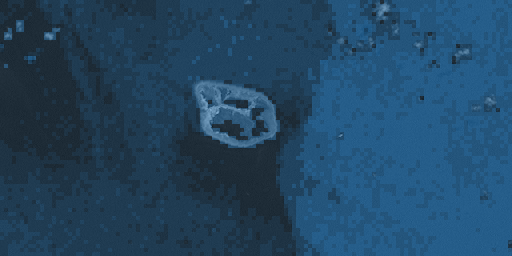
\includegraphics[width=.8\linewidth]{Figs/BKIFF_k7}
				\caption{$c=7$}
			\end{subfigure}\hfil\\
			\begin{subfigure}[h]{0.32\linewidth}
				\centering
				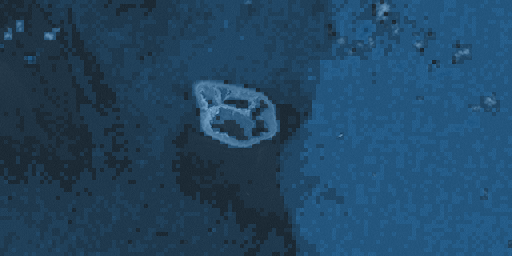
\includegraphics[width=.8\linewidth]{Figs/BKIFF_k8}
				\caption{$c=8$}
			\end{subfigure}
			\begin{subfigure}[h]{0.32\linewidth}
				\centering
				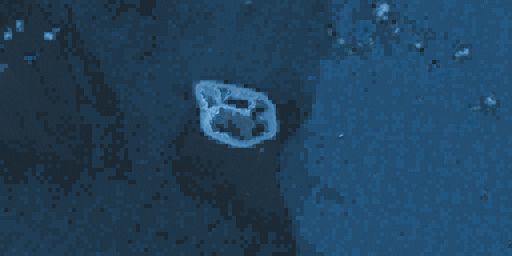
\includegraphics[width=.8\linewidth]{Figs/BKIFF_k9}
				\caption{$c=9$}
			\end{subfigure}
			\begin{subfigure}[h]{0.32\linewidth}
				\centering
				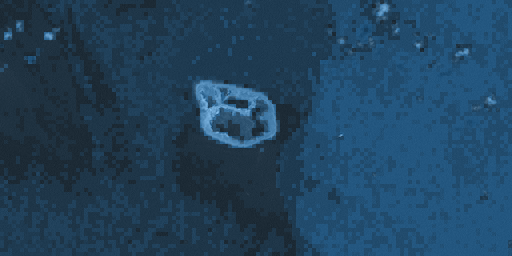
\includegraphics[width=.8\linewidth]{Figs/BKIFF_k10}
				\caption{$c=10$}
			\end{subfigure}
			\caption{Kết quả thuật toán đề nghị IFCF được áp dụng cho ảnh Landsat đối với Ví dụ~\ref{vdu:anh2}}\label{fig:APP}
			\begin{minipage}{\textwidth}
				\fontsize{11pt}{14pt}\selectfont\it
				Nguồn: Minh họa của tác giả.
			\end{minipage}
		\end{figure}
\end{frame}






\begin{frame}{3.3. Phân loại mất cân bằng (Bayes-IFCF)}{Ví dụ hình ảnh dựa vào ước lượng khối màu}
	\begin{columns}
		\begin{column}{.55\textwidth}
			
			\begin{figure}[H]
				\centering
				\begin{subfigure}{.48\textwidth}
					\centering
					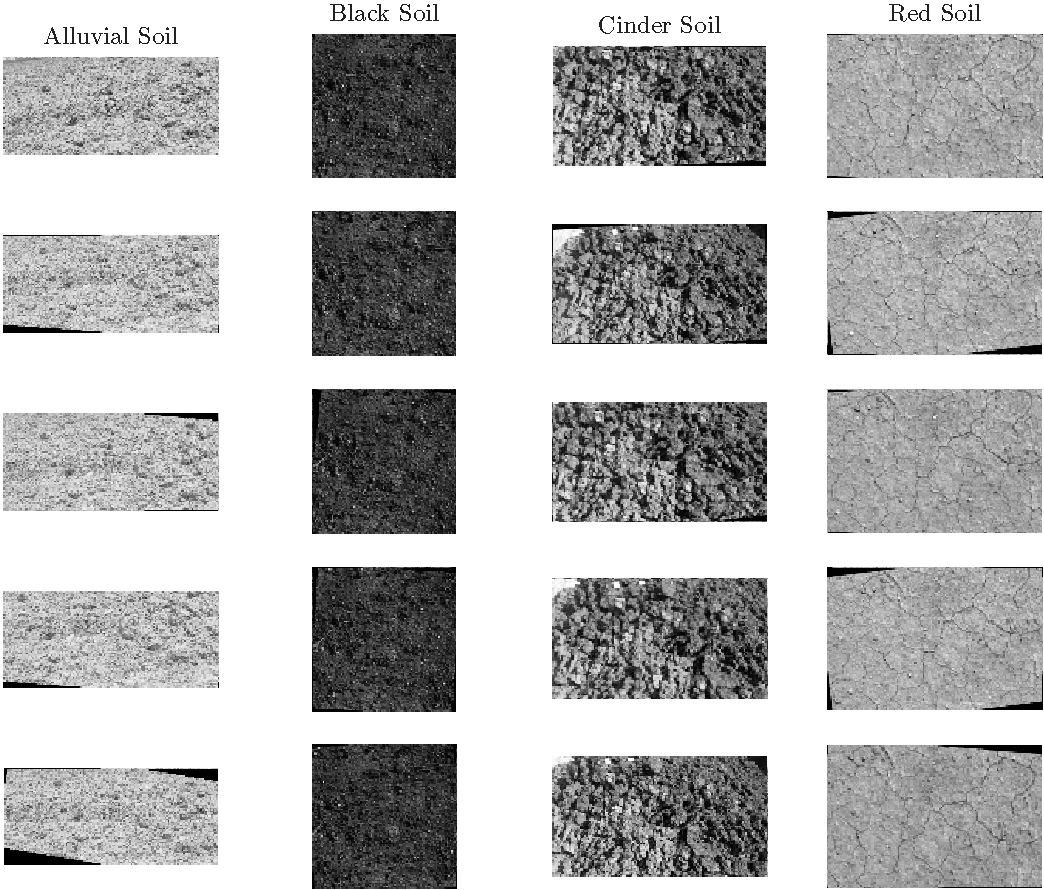
\includegraphics[width=\linewidth]{Figs/Figure_1}
					\caption{}
				\end{subfigure}
				\begin{subfigure}{.48\textwidth}
					\centering
					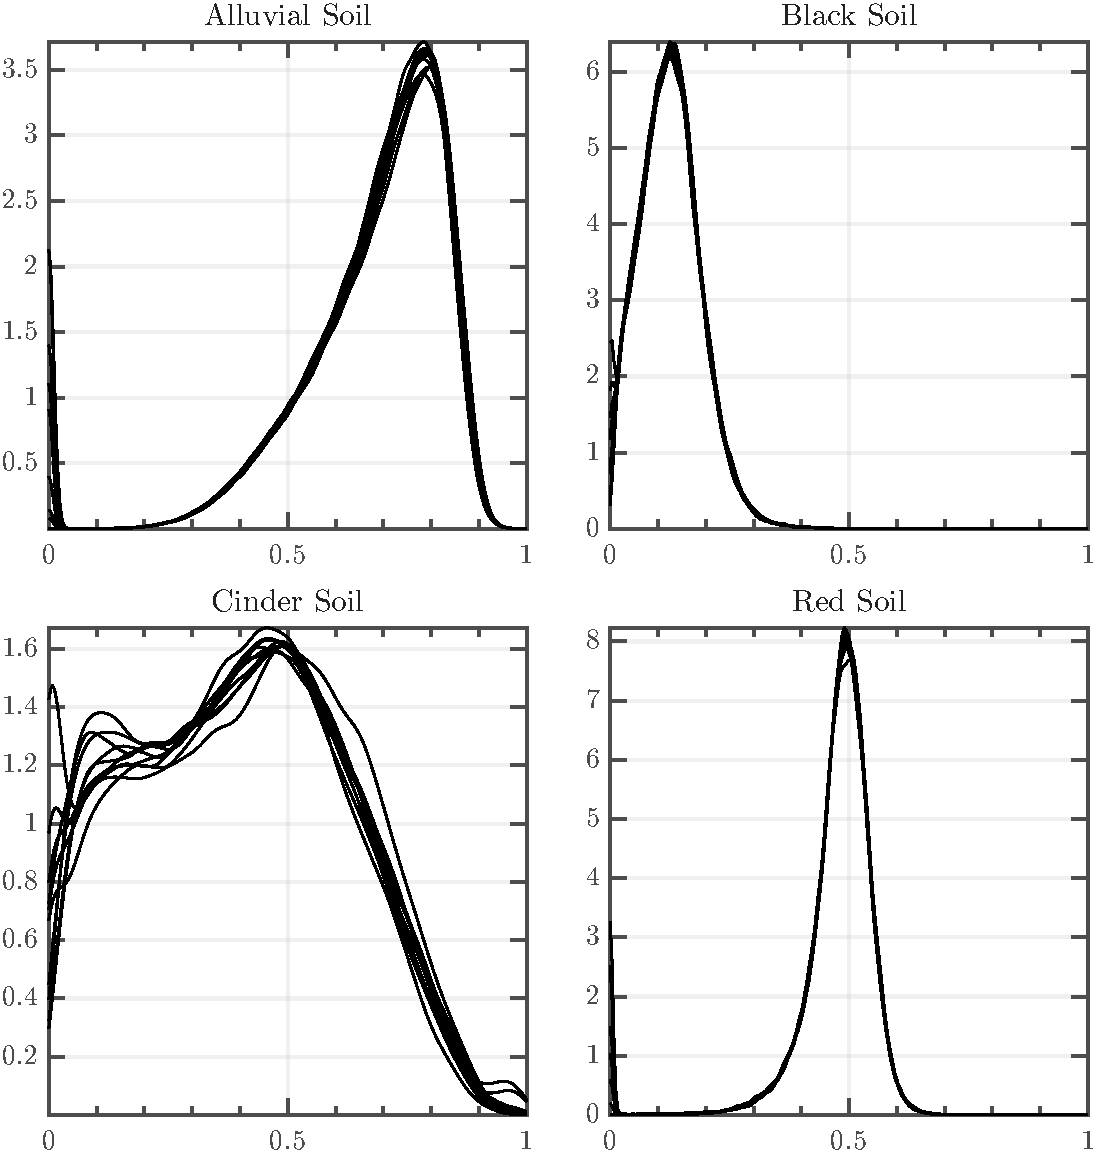
\includegraphics[width=.8\linewidth]{Figs/Figure_2}
					\caption{}
				\end{subfigure}
			\end{figure}
		\end{column}
	\end{columns}
	
	\begin{table}[H]
		\centering\scriptsize
		\begin{tabular*}{\textwidth}{@{\extracolsep\fill}llccc@{\extracolsep\fill}}
			\toprule
			Phương pháp & $ACC$ & $GM$ & $F_1$-score & Thời gian (s) \\ 
			\midrule
			Bayes-IFCF & 1{,}0$\pm$0{,}00 & 1{,}0$\pm$0{,}00 & 1{,}0$\pm$0{,}00 & 0{,}04 \\
			Bayes-FCF  & 0{,}84$\pm$0{,}12 & 0{,}37$\pm$0{,}49 & 0{,}79$\pm$0{,}16 & 0{,}14 \\
			Bayes-U    & 0{,}75$\pm$0{,}00 & 0{,}00$\pm$0{,}00 & 0{,}67$\pm$0{,}00 & 0{,}00 \\
			Bayes-L    & 0{,}50$\pm$0{,}00 & 0{,}00$\pm$0{,}00 & 0{,}38$\pm$0{,}00 & 0{,}00 \\
			Bayes-J    & 0{,}50$\pm$0{,}00 & 0{,}00$\pm$0{,}00 & 0{,}38$\pm$0{,}00 & 0{,}00 \\
			\bottomrule
		\end{tabular*}
	\end{table}
\end{frame}






{
	\usebackgroundtemplate{
\includegraphics[width=\paperwidth]{BG/thank2.pdf}}%
	\begin{frame}[plain]{}
		\vspace{1em}
		\begin{center}
			\large\bf\color{white} PHẦN KẾT LUẬN
		\end{center}
		\centering
		\begin{minipage}{.7\textwidth}
			\color{white}
			\begin{enumerate}
				\item {\color{white} Một số bàn luận}
				\item {\color{white} Kết luận và kiến nghị}
			\end{enumerate}
		\end{minipage}
	\end{frame}
}

\begin{frame}{Một số bàn luận}{Về thuật toán phân tích chùm IFCF}
				
				\begin{columns}
					\begin{column}{.4\textwidth}
						\begin{figure}[H]
							\centering
							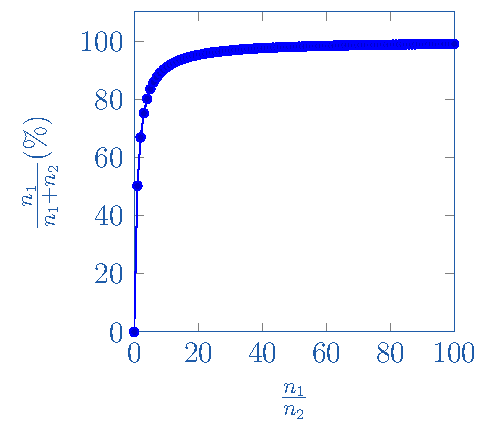
\includegraphics[width=\textwidth]{Figs/C2_hamIR}
						\end{figure}
					\end{column}
					\begin{column}{.6\textwidth}\small
							\begin{align*}
							\frac{1}{1 + \left(\frac{\omega_2}{\omega_1}\right)^{\frac{1}{m-1}}
								\left(\frac{\mathcal{L}^2_2(\theta_1\,;f_j)}{\mathcal{L}^2_2(\theta_2\,;f_j)}\right)^{\frac{1}{m-1}}}
							+
							\frac{1}{\left(\frac{\omega_1}{\omega_2}\right)^{\frac{1}{m-1}}
								\left(\frac{\mathcal{L}^2_2(\theta_2\,;f_j)}{\mathcal{L}^2_2(\theta_1\,;f_j)}\right)^{\frac{1}{m-1}}+1}
							= 1.
						\end{align*}
						Khi $\omega_1 \to \infty$, ta có $
						\lim_{\omega_1 \to \infty} \mu_{i1} = 1$ và
						$\lim_{\omega_1 \to \infty} \mu_{i2} = 0.$
					\end{column}
				\end{columns}
				
					
		
	
	
	
\end{frame}



\begin{frame}{Kết luận và định hướng nghiên cứu}\footnotesize
	
	\begin{columns}[t,onlytextwidth]
		
		% ======== CỘT TRÁI ========
		\begin{column}{0.48\textwidth}
			
			\begin{block}{\textbf{Kết luận}}
				\begin{itemize}
					\item \textbf{Phân tích chùm:} Đề xuất thuật toán mờ cải tiến \textit{IFCF} cho dữ liệu PDF mất cân bằng; được chứng minh hội tụ, tổng quát hơn các thuật toán hiện có.
					\item \textbf{Phân loại:} Thiết lập thuật toán phân loại mới với \textit{tiên nghiệm động}, dựa trên IFCF và chỉ số hậu nghiệm mới; hiệu quả hơn các tiên nghiệm tĩnh truyền thống.
					\item \textbf{Thực nghiệm:} Xây dựng quy trình trích xuất đặc trưng hình ảnh thành PDF và áp dụng hai thuật toán trên. Kết quả thực nghiệm cho thấy mô hình ổn định, chính xác, và hiệu quả tính toán cao.
				\end{itemize}
			\end{block}
			
		\end{column}
		
		% ======== CỘT PHẢI ========
		\begin{column}{0.48\textwidth}\footnotesize
			
			\begin{block}{\textbf{Định hướng nghiên cứu}}
				\textit{Về lý thuyết:}
				\begin{itemize}
					\item Phát triển mô hình SR kết hợp để xử lý hiệu ứng “đồng nhất” và “xi-phông”;
					\item Chứng minh tính hội tụ nghiêm ngặt với các $f$-phân kỳ;
				\end{itemize}
				
				\textit{Về ứng dụng:}
				\begin{itemize}
					\item Mở rộng trích xuất đặc trưng phức tạp (kết cấu, hình dạng, đa kênh màu);
					\item Tối ưu siêu tham số và phát triển công cụ XAI cho SR-PDF;
					\item Áp dụng cho dữ liệu PDF đa chiều trong các miền nghiên cứu mới.
				\end{itemize}
			\end{block}
			
		\end{column}
		
	\end{columns}
	
\end{frame}





	\section{Tài liệu tham khảo}
	
	
	\begin{frame}[allowframebreaks, noframenumbering]{Tài liệu tham khảo}
		\printbibliography
	\end{frame}
	

	
	
	\begin{frame}
		\begin{center}\color{white}
			\vspace{2cm}
			
			{\Large\color{CTUblue}\bf Chân thành cảm ơn quý Hội đồng!}\\
			[1em]
			{\color{CTUcyan} Trần Nam Hưng}	
			\vspace{1cm}

		\end{center}
		
		
	\end{frame}


{
	\usebackgroundtemplate{
\includegraphics[width=\paperwidth]{BG/out.pdf}}%
	\begin{frame}[plain]
	\end{frame}
}









\end{document}